\documentclass{mcmthesis}
\mcmsetup{CTeX = false,
          tcn = 2225971, 
          problem = D,
          sheet = true, 
          titleinsheet = true, 
          keywordsinsheet = true,
          titlepage = false, 
          abstract = false}
\usepackage{newtxtext}
\usepackage{lipsum}
\usepackage{setspace}
\usepackage{lettrine}
\usepackage{booktabs}
\usepackage{float}
\usepackage{longtable}
\usepackage{indentfirst}
\usepackage{multirow,makecell}
\usepackage[final]{pdfpages}
\setcounter{tocdepth}{2}

\newcommand{\tabincell}[2]{\begin{tabular}{@{}#1@{}}#2\end{tabular}}
%Title
\title{Analysis without Paralysis!\\
Evaluation of Maturity and Effectiveness of D\&A System}

%%Begin
\begin{document}

%Abstract
\begin{abstract}
\noindent
Viewed as a strategic asset by increasing numbers of companies, data is playing an increasingly significant role in nowadays world. However, the difficulty of extracting value from data grows as the  increase of volume and variety of data, which is called 'data paralysis'. D\&A system is built for that and we are supposed to accomplish the following 4 tasks upon it.

\noindent
Task 1 requires extracting a metric to measure the current D\&A system maturity level, considering 3 key performance indicators (KPIs). To finish the task, firstly, each KPI was divided into more detailed sub-indexes (and sub-sub-indexes) to build a comprehensive evaluation system. Then,  objective and subjective empowerment methods (AHP, EWM) are combine to get the weight of indexes, calculating the value series of 3 KPIs. And finally, we use PCA to eliminate mutual influence of these 3 series and their cross items, gaining the final expression of maturity.

\noindent
Task 2 requires demonstrating how ICM could use your model to optimize their system. Firstly, a simulation model based on Brownian motion is built and indexes series can be obtained from it easily. Using the model constructed in Task 1, we determine the maturity level and obtain its expression about the 3 KPIs. After that, two different kinds of Gradient Descent algorithms are adopted, revealing two different optimization strategies. It is concluded that the former one is faster while the latter one is easier to conduct in reality.

\noindent
Task 3 requires us to suggest steps that ICM should take to measure the effectiveness of their D\&A system. Firstly, an operational research model (OR model) is built, on the premise that the dock model is well established. Secondly, a greedy algorithm is applied to solve this complex OR model, which has a very fast speed and a relatively high precision. At most, it is 38.27\% better than a random algorithm. Based on the model and algorithm mentioned above, protocols are brought out to measure the effectiveness.

\noindent
Task4 requires the demonstration of our model applying to different scaled seaport, the analysis of the adaptation of our maturity metric to different industries. We construct a simulation model based on Poisson process, representing the events in a seaport. By changing the parameters of this simulation system, the greedy algorithm can run in different scaled seaport, comparing with the random algorithm. It turns out that our greedy algorithm is more efficient. After that, we analyze the maturity metric by inspecting three KPIs, and consider all the sub indexes. A few situations where our maturity metric fails are listed. We also analyze ICM's benefits from the promotion of maturity metric from 3 perspectives, revealing conclusions.

\noindent
Finally, we conduct sensitive analysis to inspect the influence of some specific parameters. It turns out that our system is very robust, and the influence of parameters' changing is within expectation. Furthermore, strengths, weaknesses and future work of our model are discussed.
    \begin{keywords}
         D\&A system; AHP; PCA; Gradient Descend; System Simulation
    \end{keywords}
\end{abstract}
\maketitle

%Content
% \begin{spacing}{0.1}
    \tableofcontents
% \end{spacing}
\newpage

%Introduction
\section{Introduction}
\subsection{Background Research}
\lettrine[lines=2]{I}{n} recent years, data has been viewed as a strategic asset by increasing numbers of companies, which could Improve the efficiency and profitability of company operations. However, it has been more and more difficult to derive value from this asset, as the growth of size and variety of data\cite{1}, which is called 'data paralysis'. 

Proper management of this precious resource can lead to a competitive advantage. Thus, an integrated data and analytics (D\&A) system is urgently required, where companies can guarantee that they have the right people, technologies, and processes in place to manage, manipulate, use, and protect this resource. According to literature, people, technologies and processes are three key components of D\&A system, so how to ensure the reliability of people, technologies and processes is the core of establishing D\&A system and the main concern when evaluating D\&A system.

\subsection{Problem Restatement}
Our team was hired by the Intercontinental Cargo Moving (ICM) Corporation to measure the maturity of their current D\&A system and provide a solid plan to optimize their D\&A capabilities. We are supposed to develop a model to evaluate the D\&A system of ICM Corporation and the model development and report should cover the following requirement:
\begin{itemize}
    \item A metric to measure the current D\&A system maturity level for ICM Corporation. Include key performance indicators that measure the success of their D\&A people, technologies, and processes;
    \item A demonstration on how ICM corporation could use the model to recommend changes to the system allowing the company to maximize the potential of their data assets;
    \item Protocols that ICM should put in place to measure the effectiveness of their D\&A system;
    \item A demonstration of how the model might be applied to a larger or smaller seaport, and how the system maturity metric will be extended to be adapted to other industries. Specifically, use the maturity metric for a trucking company as a customer of ICM and explain how this could benefit ICM Corporation.
\end{itemize}

\subsection{Overview of Our Work}
For task 1, we establish the evaluation index system for people, technology and process, and use EWM-AHP method to calculate the evaluation value. After comprehensively considering the interaction among the three indicators, we established a quantitative evaluation model of D\&A system using PCA method.

For task 2, we present a constrained optimization model and use the gradient descent strategy to find the system improvement strategy. We also designed a simulation system to demonstrate the solution process and results of the model.

For task 3, we first established a cargo scheduling model to optimize the optimal residence time, and defined the effectiveness of the D\&A system by comparing the actual residence time with the optimal time. The main factors affecting effectiveness were observed through solving the model, and the rationalization protocols were given accordingly

For task 4, we show the optimization results of the scheduling model in three different sizes of ports, and consider the application and promotion of the model in other fields.

In order to demonstrate our work clearly, we present the overview of the paper by  Figure \ref{figure::Demonstration of Our Work}.

\begin{figure}[!htbp]
    \small
    \centering
    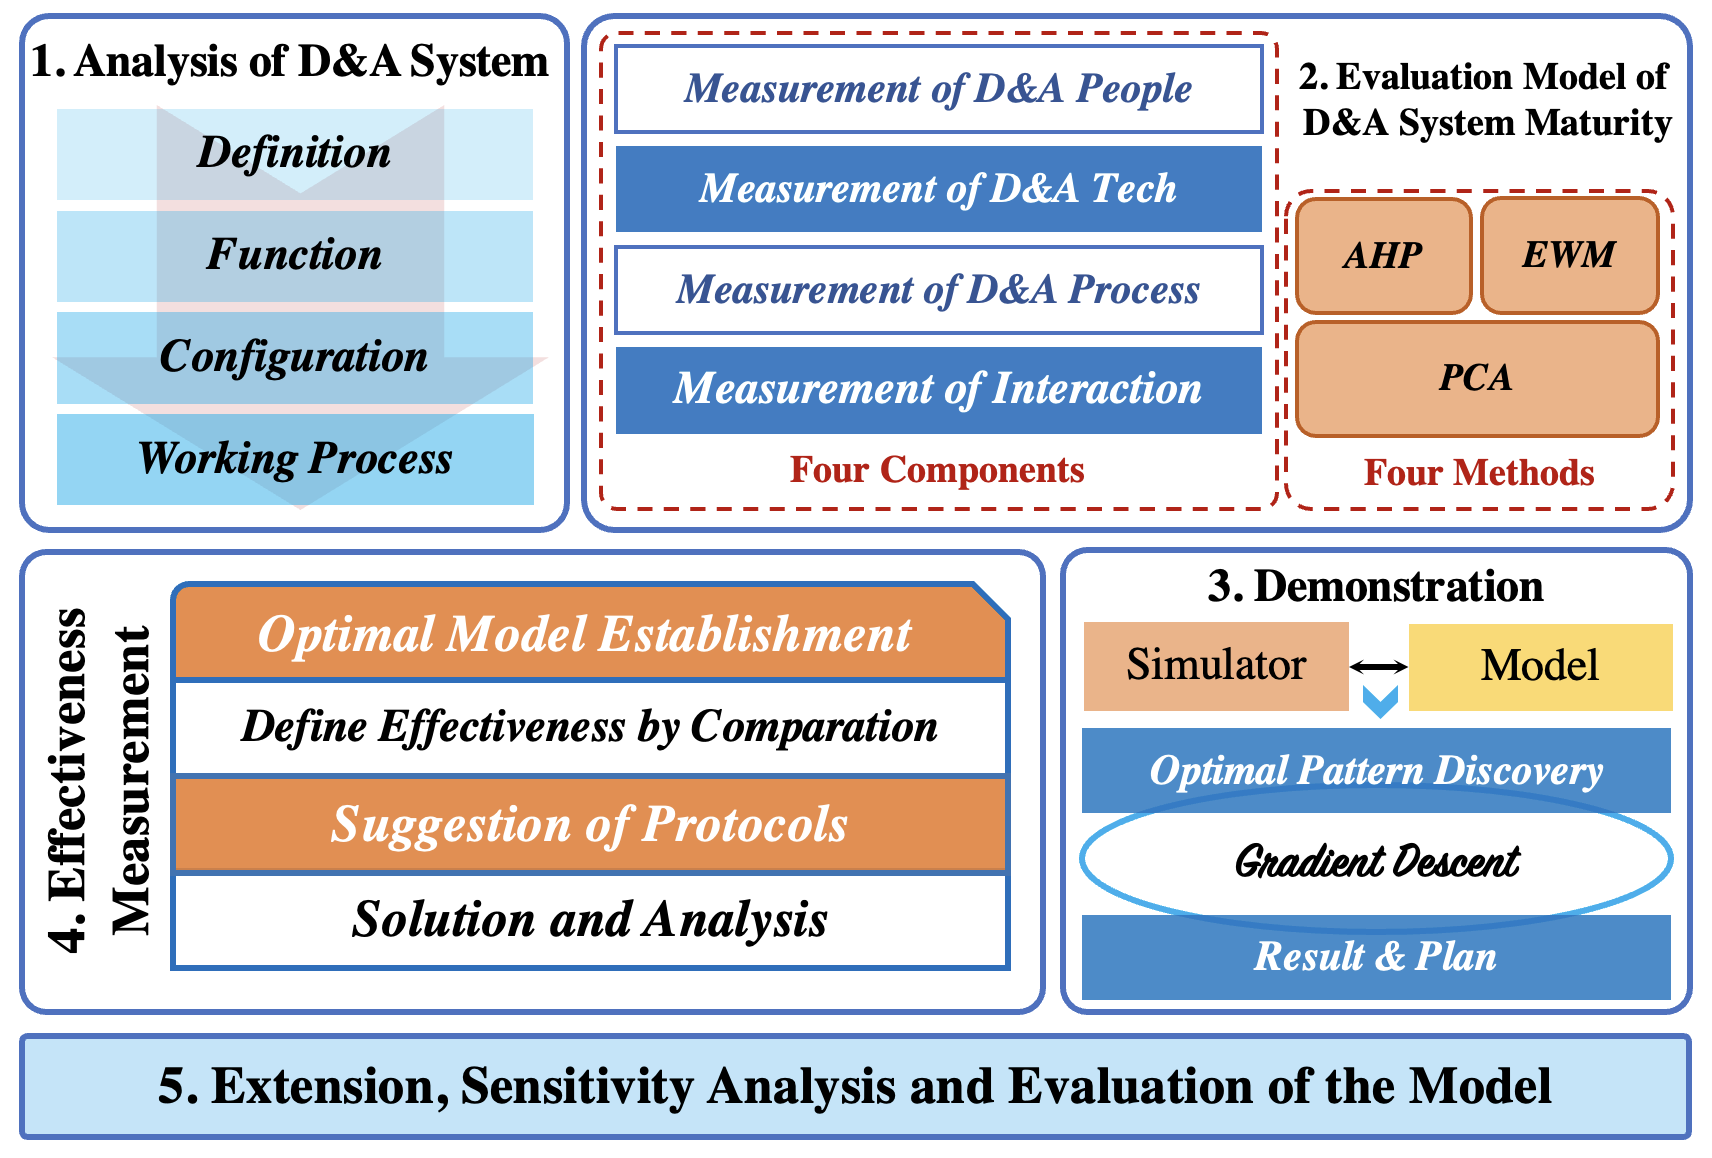
\includegraphics[width=15cm]{figures/DemonstrationofOurWork.png}
    \caption{Demonstration of Our Work} 
    \label{figure::Demonstration of Our Work}
\end{figure}%figure::Demonstration of Our Work

%Model Preparation
\section{Model Preparation}
\subsection{Notations}
We'd like to begin by defining a list of the notations used in the paper as Table \ref{table::Notations}.

\begin{table}[!htbp]
    \small
    \setlength{\abovecaptionskip}{0cm}
    \setlength{\belowcaptionskip}{+0.1cm}
    \caption{Notations}
    \label{table::Notations}
    \centering
    \begin{tabular}{cl}  
    \toprule   
    \textbf{Abbreviation} & \textbf{Description}\\  
    \midrule
    $PE(t)$,$M_{PE}(t)$ & Indicator set and maturity of D\&A people \\
    $TE(t)$,$M_{TE}(t)$ & Indicator set and maturity of D\&A technologies \\
    $PR(t)$,$M_{PR}(t)$ & Indicator set and maturity of D\&A processes \\
    $M(t)$ & Measurement of the maturity of D\&A system \\
    $CI$ & Consistency index in AHP\\
    $RI$ & Random consistency index in AHP\\
    $CR$ & Consistency Ratio in AHP\\
    $\eta$ & Step size in the iteration\\
    $TD,TA$ & Leaving and arriving time of a vehicle\\
    $EFF(i,j)$ & Effectiveness of D\&Asystem in the period of $(i,j)$\\

    \bottomrule  
    \end{tabular}
\end{table}%table:Notations

\subsection{Assumptions and Justifications}
To simplify the problem and make it convenient for us to simulate real-life conditions, we make the following basic assumptions, each of which is properly justified.

\begin{itemize}
\item ICM corporation has all the data needed in our evaluation model. This paper considers the way to get every index for ICM corporation, which isn't considered to be hard. 
\item We consider all customs inspection reports to be true.
\item We consider the time for any container's transfer using any tower crane to anywhere to be same. And we omit the time that tower cranes move around.
\item Time interval between ships/trucks/trains arriving at the port is independent of each other and obeys Poisson distribution
\end{itemize}


%Task 0
\section{Brief Description of D\&A System}
D\&A system plays an important role in managing data assets and is what we are trying to optimize. In this section, we will give a brief description of the D\&A system including its universal definition, function and configuration, which will be a foundation of our model.

\subsection{Defination and Function}
Data and analytics system, abbreviated as D\&A System, is a significant department that collects, statistics, manages and analyzes the data generated in the process of enterprise operation, mines the valuable information contained in the data, puts forward feasible suggestions for enterprise operation and improves the efficiency of enterprise operation and management. In ICM Corporation, an effective D\&A system ensures the process is efficient so that the time a ship, truck, or train spends at the port is minimized.

\subsection{Configuration}
A D\&A System mainly consists of three components—people, technology, and process. Together with the operation system, HR department, IT department and ISO department, the main part of the ICM Corporation is establishment. 

\begin{figure}[!htbp]
    \small
    \centering
    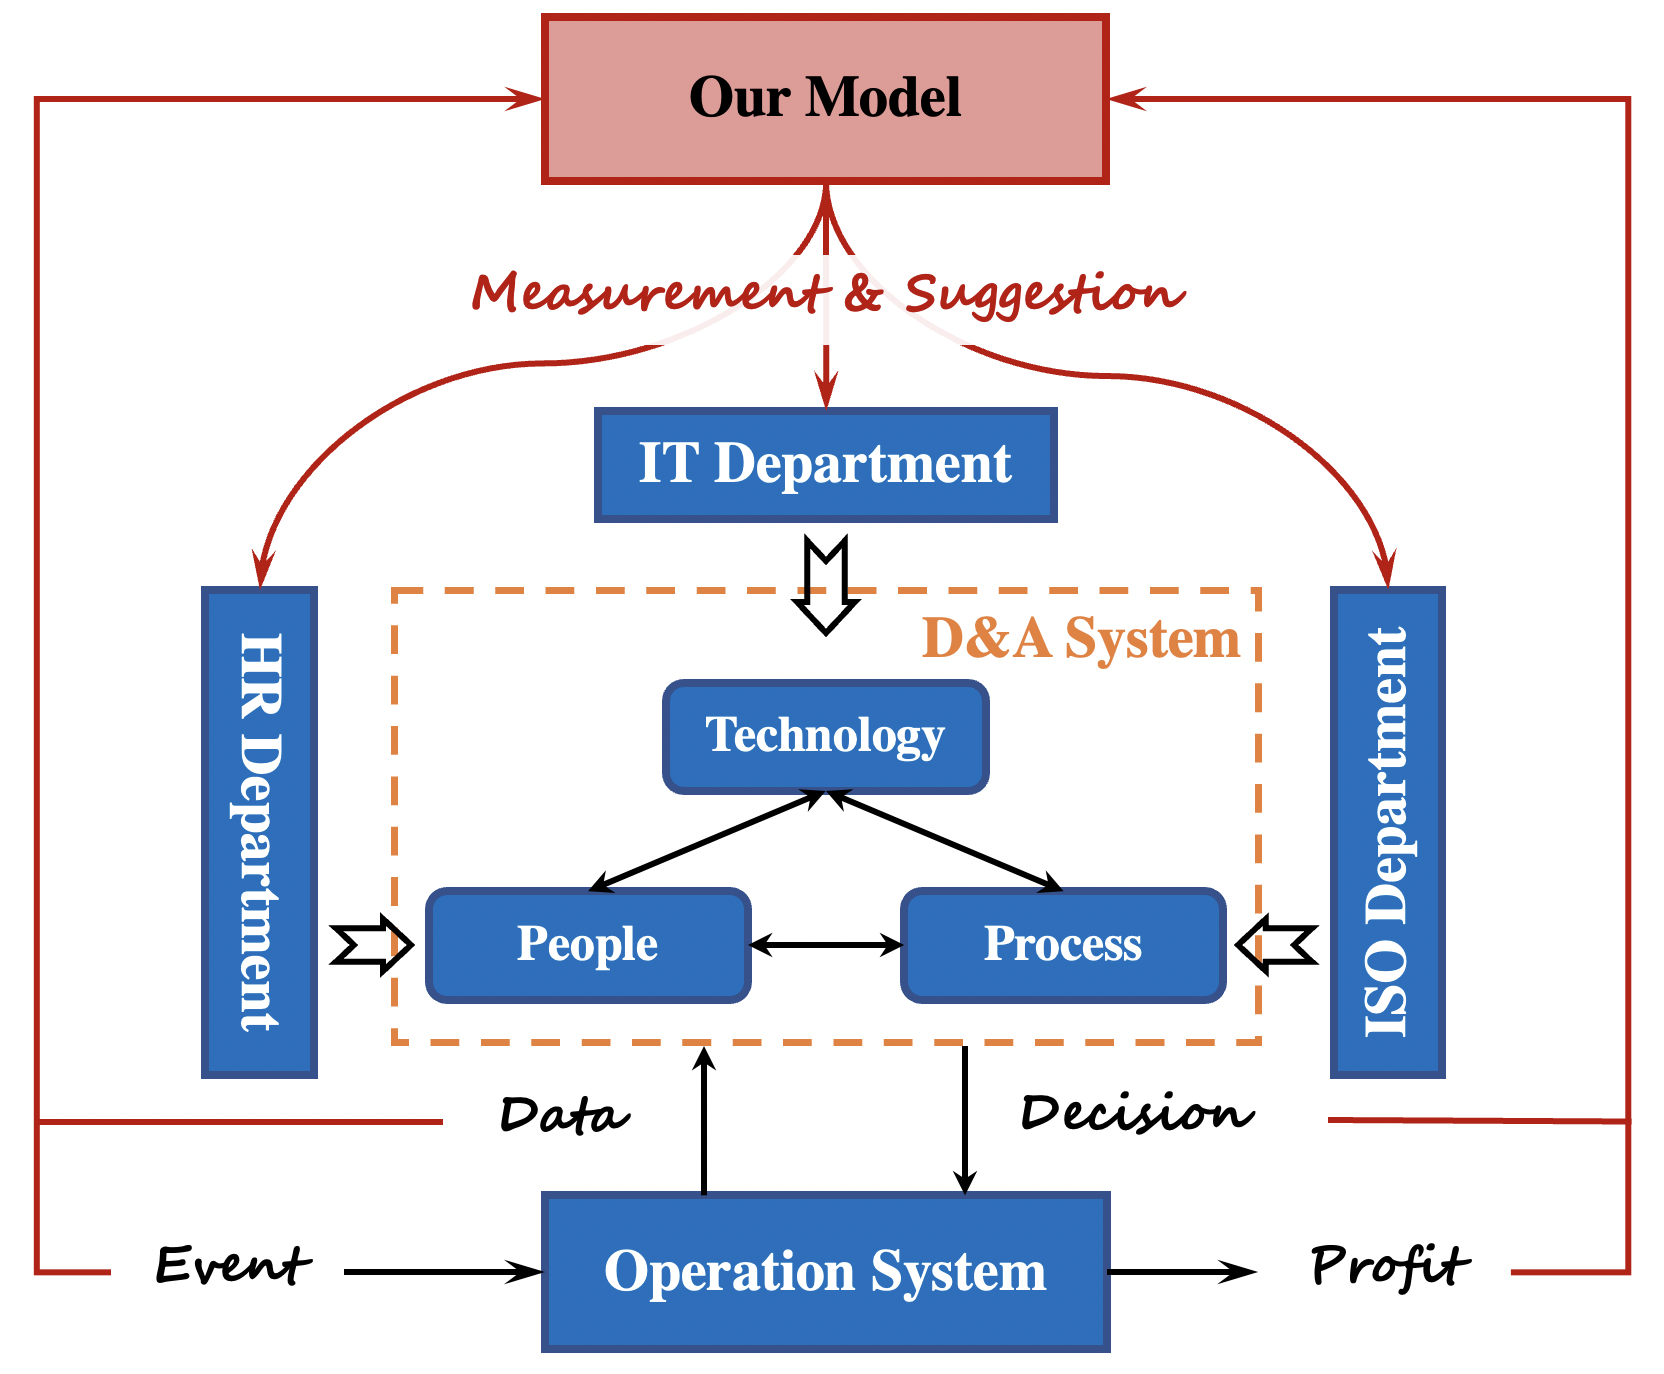
\includegraphics[width=10cm]{figures/StructureofICMCorporation.png}
    \caption{Structure of ICM Corporation} 
    \label{figure::Structure of ICM Corporation}
\end{figure}%figure::Structure of ICM Corporation

Figure \ref{figure::Structure of ICM Corporation}  clearly displays how the corporation is working. The operation system generates revenue for the company by processing business, during which a large amount of data is generated. These data will be analyzed and processed by D\&A system, so as to feedback reasonable suggestions and decisions to operation system. 

Three important departments were built as the supervisor of D\&A system. Hiring managers need to consider multiple factors in hiring qualified D\&A talent. The Information Technology (IT) department needs a way to measure the effectiveness of technology solutions now and in the future. The Information Security Officer (ISO) is concerned about the D\&A processes that are in place to protect and manage the data. 

Thus, our model is required to be established to provide measurement of maturity of D\&A system and give the proper suggestions for the departments mentioned above according to the information generated during the whole process of system operation.


%Task 1
\section{\scshape{Task 1:} \upshape{D\&A System Maturity Level Measurement}}
In order to help ICM Corporation optimize their analytic capabilities, obtain a competitive advantage, and give customers confidence in the company’s ability to manage data, developing a model to measure the maturity of the D\&A System is necessary.

To maximize the potential of their data assets, companies want highly skilled people, relevant technologies, mature processes, and a strong connection among all three components. In the following parts, the measurement of D\&A people, technologies, process, and their interaction is introduced.  These constitute the basis for us to choose evaluation indicators and build the maturity evaluation system.

In this section, we will display our work about the establishment of the maturity evaluation model, including four main sub-models, which, respectively, are the measurement of people based on EWM-AHP, measurement of technologies based on AHP, measurement of processes based on AHP and interaction among them based on PCA. We finally provide a comprehensive evaluation model of the maturity of D\&A system, and list the detailed methods to use it.

\subsection{Measurement of the Success of D\&A People}
\subsubsection{Indicators Selection}

According to the literature, we build the indicator system of the measurement of people as shown in Figure \ref{figure::Measurement Indicators of People}. The assessment criteria of a talent can be mainly divided into quality ($pe_1$) and performance ($pe_2$), while quality has sub indexes ideological quality ($a_1$), intelligence quotient ($a_2$), emotional intelligence ($a_3$), physiological quality ($a_4$), and performance has sub indexes work quantity ($b_1$), work quality ($b_2$), work efficiency ($b_3$). Considering the question, two additional indexes, rationality of Individuals number ($pe_3$) and professional degree ($pe_4$), are added. 

These four quality sub indexes can be quantified by taking exams, which we suppose the ICM corporation has owned the staff is employed. These three performance sub indexes can be quantified by the department heads. And rationality of Individuals Number can be defined as
$pe_3 = 1-n/N$, where $n$ is the actual individual number and $N$ is the optimal individual number, according to literature. Anyhow, it is reasonable to assume that the ICM corporation has all the data at any specific time needed in this evaluation model. To simplify, at this stage, time span is not considered, and all the indexes reflect the D\&A people's condition at a specific time. And they are standardized.

\begin{figure}[!htbp]
    \small
    \centering
    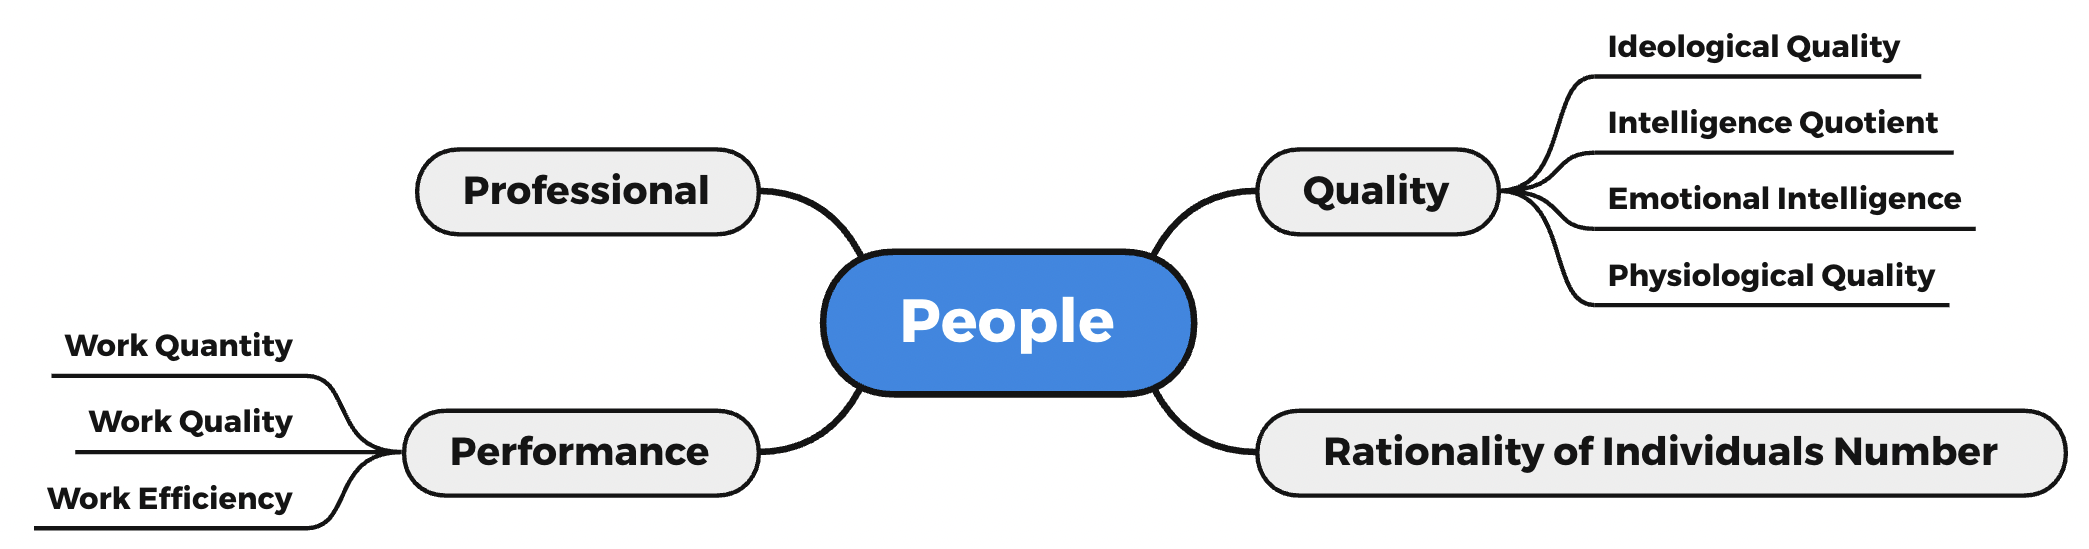
\includegraphics[width=12cm]{figures/IndicatorsofPeople.png}
    \caption{Measurement Indicators of People} 
    \label{figure::Measurement Indicators of People}
\end{figure}%figure::Measurement Indicators of People

For the convenience of the evaluation, we define indicator set of people $PE(t)$ and the set of the weight of each indicator $W_{PE}(t)$ as shown in Formula \ref{formula::pe} and \ref{formula::wpe}.
\begin{equation}
    PE(t)=[pe_1,pe_2,pe_3,pe_4]
    \label{formula::pe}
\end{equation}
\begin{equation}
    W_{PE}(t) = [w_{pe1},w_{pe2},w_{pe3},w_{pe4}]
    \label{formula::wpe}
\end{equation}

\subsubsection{Combinations of Sub-indicators Based on EWM}
First we use the EWM method to make the combination of the sub-indicators of the index $pe_1$ (quality) and $pe_2$ (performance). The entropy weight method (EWM) is an important information weight model, whose biggest advantage is the weights are generated by measuring the degree of differentiation, rather than subjectively created.

With the EWM, when there are $m$ indicators and $n$ samples set in the evaluation, we record $x_{ij}$ as the measured value of the $i$th index in the $j$th sample. After normalize $x_{ij}$ with Formula \ref{formula::pij}, we get the standardized value of the $i$th index in the $j$th sample noted as $p_{ij}$\cite{2}.
\begin{equation}
    p_{ij}=\frac{x_{ij}}{\sum_{j=1}^n x_{ij}}
    \label{formula::pij}
\end{equation}

The entropy value $E_i$ of the $i$th index is defined as
\begin{equation}
    E_i = - \frac{ \sum_{j=1}^n p_{ij} \ln p_{ij} }{\ln n}
\end{equation}  
whose value range is $[0,1]$. As definition, the index sharing larger $E$ will share a higher weight during the evaluation. Therefore, in the EWM, the calculation method of weight $w_i$ of the $i$th index is defined as
\begin{equation}
    w_i = \frac{1-E_i}{\sum_{i=1}^m(1-E_i)}
\end{equation}
    
By using the EWM, the weight of Ideological quality, Intelligence quotient, Emotional intelligence, Physiological quality to quality, and the weight of Work quantity, Work quality, Work efficiency to performance, can then be obtained. Then, the value of quality and performance can be calculated using Formula \ref{formula::quality} and \ref{formula::performance}.
\begin{equation}
    pe_1 = w_1a_1+w_2a_2+w_3a_3+w_4a_4
    \label{formula::quality}
\end{equation}
\begin{equation}
    pe_2 =w_5b_1+w_6b_2+w_7b_3
    \label{formula::performance}
\end{equation}

\subsubsection{Measurement of D\&A People Based on AHP}
We use Analytic Hierarchy Process (AHP) to measure the relationship between $M_{PE}$ and $PE = [pe_1,pe_2,pe_3,pe_4]$.

By searching keywords 'talents \& quality', 'talents \& performance', 'talents \& rationality of Individuals number', and 'talents \& technical adaptability', we get 856{,}000, 607{,}000, 4{,}270{,}000 and 772{,}000 results respectively, which embodies the importance of each index. Using the data above, the comparison matrix can be approximately constructed as follows,
\begin{equation}
    \setlength{\arraycolsep}{5pt}
    C = (c_{ij})_{4 \times 4} = \begin{bmatrix}
    1 & 3 & \frac{1}{2} & 2\\[1mm]
    \frac{1}{3} & 1 & \frac{1}{7} & \frac{1}{2} \\[1mm]
    2 & 7 & 1 & 4 \\[1mm]
    \frac{1}{2} & 2 & \frac{1}{4} & 1 \\
    \end{bmatrix}
\end{equation}

Construct the judgment matrix $(d_{ij})_{4 \times 4}$, and
\begin{equation}
d_{ij} = \begin{cases}
\frac{r_i-r_j}{r_{\max}-r_{\min}}(d_m-1)+1, r_i \geq r_j \\[2mm]
[\frac{r_i-r_j}{r_{\max}-r_{\min}}(d_m-1)+1]^{-1}, r_i \leq r_j 
\end{cases}
\end{equation}
where $r_i=\sum_{i=1}^4 c_{ij}$,$d_m = r_{\max} / r_{\min}$. And the maximum eigenvalue $\lambda_{\max}$ could be calculated by
\begin{equation}
    \lambda_{\max} = \frac{1}{4} \sum_{i=1}^4 \frac{(Dq)_i}{q_i}
\end{equation}
where $q_i = \sqrt{\prod_{j=1}^4 d_i}/ \sum_{i=1}^m \sqrt{\prod_{j=1}^4 d_i}$.

To make the consistency test, we calculate
\begin{equation}
    CR = \frac{CI}{RI}
\end{equation}
where 
\begin{equation}
    CI = \frac{\lambda_{\max}-n}{n-1}
\end{equation}
and $RI$ is the the average random consistency index. When $CR < 0.1$, the judgment matrix is considered to meet the consistency requirements. Otherwise, the judgment matrix should be adjusted until it meets the consistency test requirements\cite{3}.

In the measurement of D\&A people, the detailed result is shown in Table \ref{table::Results of AHP Analysis}. 

\begin{table}[!htbp]
    \small
    \setlength{\abovecaptionskip}{0cm}
    \setlength{\belowcaptionskip}{+0.1cm}
    \caption{Results of AHP Analysis}
    \label{table::Results of AHP Analysis}
    \centering
    \begin{tabular}{ccccccc}  
    \toprule   
    \textbf{Indexes} & \textbf{Eigenvectors} & \textbf{Weights} & \textbf{Max\_eigenvalue} & \textbf{CI} & \textbf{RI} & \textbf{CR} \\
    \midrule
    \textbf{$pe_1$} & 1.3161 & 0.2555 & \multirowcell{4}{4.0078} & \multirowcell{4}{0.0026} & \multirowcell{4}{0.8820} & \multirowcell{4}{0.0029}\\
    \textbf{$pe_2$} & 0.3928 & 0.0763 \\
    \textbf{$pe_3$} & 2.7356 & 0.5310 \\
    \textbf{$pe_4$} & 0.7071 & 0.1373 \\   
    \bottomrule
    \end{tabular}
\end{table}%table::Results of AHP Analysis

As the maximum eigenvalue of 4.0078 and the consistency ratio  $CR = 0.0029$, the result meets the requirements of AHP successfully. Therefore, the calculation method of the success of D\&A people is obtained, as shown in Formula \ref{formula::people}.
\begin{equation}
    \begin{split}
    M_{PE}(t) &= W_{PE}(t) \cdot PE(t)^T \\
              &= 0.2557pe_1+0.0764pe_2+0.5305pe_3+0.1374pe_4
    \end{split}
    \label{formula::people}
\end{equation}


\subsection{Measurement of the Success of D\&A Technologies}
\subsubsection{Indicators Selection}
We selected five factors to evaluate the success of the D\&A technologies as shown in Figure \ref{figure::Measurement Indicators of Technologies}. The first is the industry leading degree of technology ($te_1$). It reflects whether the technology has high productivity and advanced level.The second and third are reliability ($te_2$) and flexibility ($te_3$), which can reflect whether it can reduce the occurrence of faults and work normally in different complex environments. Scalability ($te_4$) reflects whether the system can be upgraded and expanded with new functions, as well as the development potential. Security ($te_5$) is also important. The more secure the system is, the less vulnerable it is to hacker attacks. Correspondingly, the disclosure of trade secret data is less likely to happen. 

\begin{figure}[!htbp]
    \small
    \centering
    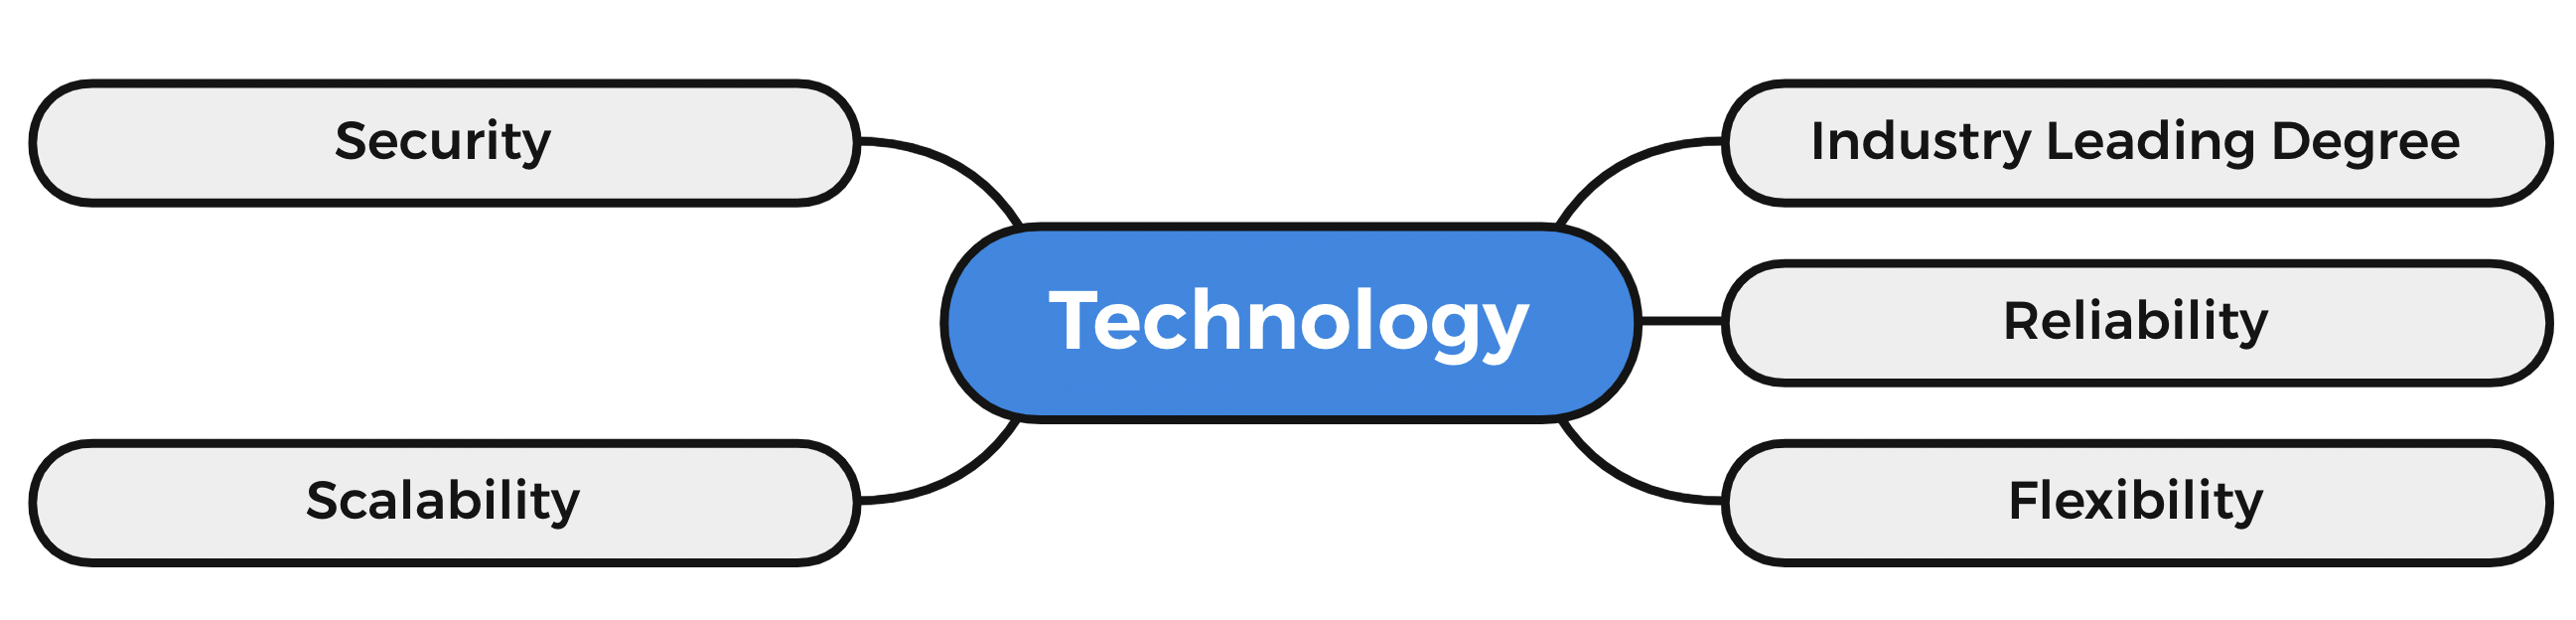
\includegraphics[width=12cm]{figures/IndicatorsofTechnology.png}
    \caption{Measurement Indicators of Technologies} 
    \label{figure::Measurement Indicators of Technologies}
\end{figure}%figure::Measurement Indicators of Technologies

For the convenience of the evaluation, we define indicator set of technology $TE(t)$ and the set of the weight of each indicator $W_{TE}(t)$ as shown in Formula \ref{formula::te} and \ref{formula::wte}.
\begin{equation}
    TE(t) = [te_1,te_2,te_3,te_4,te_5]
    \label{formula::te}
\end{equation}
\begin{equation}
    W_{TE}(t) = [w_{te1},w_{te2}, \dots ,w_{te6}]
    \label{formula::wte}
\end{equation}

\subsubsection{Measurement of D\&A Technologies Based on AHP}
Using the AHP method described in Section 4.2.3, we integrate the six indicators in the performance category and determine the weight of each indicator. The maximum eigenvalue is 5.0186 and the consistency ratio  $CR = 0.0042$, which meets the requirements of AHP successfully. Then the calculation method of the success of D\&A people is obtained as shown in Formula \ref{formula::technology}.
\begin{equation}
    \begin{split}
    M_{TE}(t) &= W_{TE}(t) \cdot TE(t)^T \\
              &= 0.1852te_1+0.3256te_2+0.0392te_3+0.1077te_4+0.3424te_5
    \end{split}
    \label{formula::technology}
\end{equation}


\subsection{Measurement of the Success of D\&A Processes}

\subsubsection{Indicators Selection}
According to the literature, six indicators are introduced to measure the success of processes as shown in Figure \ref{figure::Measurement Indicators of Processes}, which are transparency ($pr_1$), efficiency ($pr_2$), controllability ($pr_3$), timeliness ($pr_4$) , security ($pr_5$) and consistency ($pr_6$).

\begin{figure}[!htbp]
    \small
    \centering
    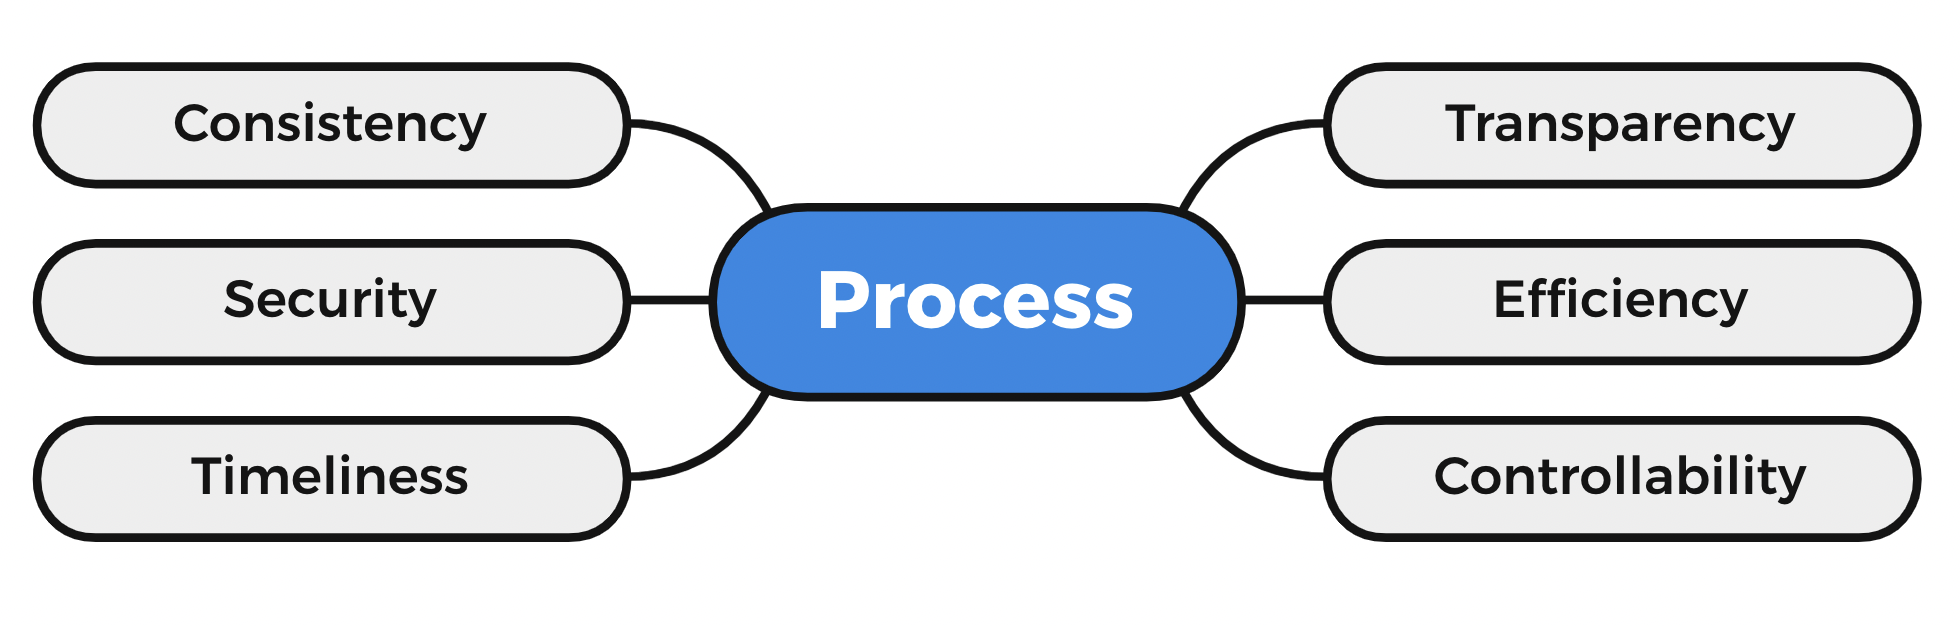
\includegraphics[width=10cm]{figures/IndicatorsofProcess.png}
    \caption{Measurement Indicators of Processes} 
    \label{figure::Measurement Indicators of Processes}
\end{figure}%figure::Measurement Indicators of Processes

For the convenience of the evaluation, we define indicator set of process $PR(t)$ and the set of the weight of each indicator $W_{PR}(t)$ as shown in Formula \ref{formula::pr} and \ref{formula::wpr}.
\begin{equation}
    PR(t) = [pr_1,pr_2,pr_3,pr_4]
    \label{formula::pr}
\end{equation}
\begin{equation}
    W_{PR}(t) = [w_{pr1},w_{pr2}, \dots ,w_{pr6}]
    \label{formula::wpr}
\end{equation}

\subsubsection{Measurement of D\&A Processes Based on AHP}
Here, AHP is introduced again, by executing the steps just like that in Section 4.2.3. As the maximum eigenvalue is 6.0418 and the consistency ratio  $CR = 0.0067$, which meets the requirement of AHP, the formula for calculating the success of D\&A processes can be obtained, which is shown in Formula \ref{formula::process}.
\begin{equation}
    \begin{split}
    M_{PR}(t) &= W_{PR}(t) \cdot PR(t)^T \\
              &= 0.2357pr_1+0.6675pr_2+0.3704pr_3+0.5818pr_4+0.0746pr_5+0.1328pr_6
    \end{split}
    \label{formula::process}
\end{equation}


\subsection{Interaction among People, Technologies and Processes}

In the mathematical sense, the value of each index of the model can increase without limit so as to make the evaluation index become better without limit, which is impossible in the practical sense. Therefore, in addition to the correlation of different indicators, constraint conditions also need to be considered and added into the evaluation model.

In fact, under the restriction of capital, environment, technology and other conditions, the growth of each indicator has its upper and lower bounds, and when one indicator grows, the growth of other indicators may be affected due to the restriction of conditions.

However, since we cannot obtain real data or the specific operation process of the D\&A system, it is difficult to describe this constraint quantitatively, so we describe these constraints as
\begin{equation}
    \begin{cases}
    L_{M_{PE}} \leq M_{PE} \leq H_{M_{PE}} \\
    L_{M_{TE}} \leq M_{TE} \leq H_{M_{TE}} \\
    L_{M_{PR}} \leq M_{PR} \leq H_{M_{PR}} \\
    f(M_{PE},M_{TE},M_{PR}) \leq C
    \end{cases}
\end{equation}
where $L,H,C$ are constants.

By considering the past time series of the three variables, the influence can be revealed by using PCA method with real data, which is shown in the next part.

\subsection{Comprehensive Evaluation Model Construction}

\subsubsection{Principal Component Analysis}
In Section 4.4, we have exam interaction among people, technologies and processes. Apart from people, technologies and processes, people$\times$technologies, people $\times$ processes, technologies $\times$ processes and people $\times$ technologies $\times$ processes are added to the model to reflect the interaction. 

Considering the possible duplication of information, we choose Principal Component Analysis(PCA) method to study the contribution of these seven factors, which is seen as a powerful algorithm for data dimension reduction. After analyzing and ranking the seven factors, it is expected to find the factors that play a major role. The specific process is introduced as follows.

As the analysis in the former part, we note the 7-dimensional standardized evaluation indicators as
\begin{equation}
    \begin{split}
    X =& [x_1,x_2,x_3,x_4,x_5,x_6,x_7] \\
    =& [M_{PE},M_{TE},M_{PR},M_{PE} \cdot M_{TE},M_{TE} \cdot M_{PR},M_{PR} \cdot M_{PE},M_{PE} \cdot M_{TE} \cdot M_{PR}]
    \end{split}
\end{equation}

According to the PCA methods\cite{4}, firstly, we define the correlation coefficient matrix of the D\&A system evaluation indexes to be
\begin{equation}
    R = (r_{ij})_{7 \times 7}
\end{equation}
and
\begin{gather}
    r_{ij} = \frac{\sum_{k=1}^n a_{ki} \cdot a_{kj}}{n-1},i,j=1,2,\dots,7 \\
    r_{ii}=1,r_{ij}=r{ji} \notag
\end{gather}
where $r_{ij}$ is the correlation coefficient between index $i$ and index $j$, $a_{ij}$ is the standardized value of the $j$th index of the $i$th sample.

Next, calculate the eigenvalues $\lambda_1 \geqslant \lambda_2 \geqslant \dots \geqslant \lambda_7$ and the eigenvectors $\mathbf{u_1},\mathbf{u_2},\dots,\mathbf{u_7}$ of the correlation coefficient matrix $R$, where
\begin{equation}
    \mathbf{u_j}=[u_{1j},u_{2j},\dots,u_{5j}]^T
\end{equation}

Seven new supplier evaluation variables are composed of feature vectors
\begin{equation}
    \begin{cases}
    y_1 = u_{11}x_1+u_{21}x_2+\dots +u_{71}x_7 \\
    y_2 = u_{12}x_1+u_{22}x_2+\dots +u_{72}x_7 \\
    \dots \\
    y_1 = u_{17}x_1+u_{27}x_2+\dots +u_{77}x_7 
    \end{cases}
    \label{formula::yy}
\end{equation}
where $y_1$ is the first principal component, $y_2$ is the second principal component, etc. The D\&A system is evaluated from seven dimensions, and the information contribution rate and cumulative contribution rate of eigenvalues are calculated by
\begin{equation}
    b_j=\frac{\lambda_j}{\sum_{i=1}^7 \lambda_k}
\end{equation}
where $b_j$ is called the information contribution rate of the main component. And the cumulative contribution rate of principal components is
\begin{equation}
    \alpha_p = \frac{\sum_{k=1}^p \lambda_k}{\sum_{k=1}^7 \lambda_k}
\end{equation}

When $\alpha_p$ is close to 1, the first $p$ evaluation index variables are selected as P principal components, and there is the final comprehensive evaluation score model
\begin{equation}
    M = \sum_{j=1}^p b_jy_j
    \label{formula::MM}
\end{equation}

The higher the comprehensive evaluation score $M$, the better the comprehensive evaluation, indicating that the index is more important.

\subsubsection{Final Evaluation Model of D\&A System}

Make an expansion of Formula \ref{formula::MM} by Formula \ref{formula::yy}, we get the final evaluation model of D\&A system as
\begin{equation}
    \begin{split}
    M(t) &= w_1M_{PE}+w_2M_{TE}+w_3M_{PR} \\
    &+w_4M_{PE} \cdot M_{TE} +w_5M_{TE} \cdot M_{PR} +w_6M_{PR} \cdot M_{PE} \\
    &+w_7M_{PE} \cdot M_{TE} \cdot M_{PR}   
    \end{split}
    \label{formula::Mt}
\end{equation}

When using the model, statistics are needed to calculate the weight of each indicators and limitation of the constraints among indicators is needed to concern. We will give a detailed demonstration of using the model in the next section.

%Task 2
\section{\scshape{Task 2:} \upshape{Model Demonstration and Optimization}}
In this section, we mainly show how to use the maturity evaluation model established in Section 4 to solve practical problems. In order to simulate the real application environment and obtain the necessary data, we first establish a simulation system using the stochastic process method to simulate the personnel change, technical innovation and process improvement in the real situation. Then we applied the evaluation model to the simulation system to demonstrate the process of calculating maturity according to the real data and proposing improvement schemes.

\subsection{Establishment of Simulation System}

\subsubsection{Structure}
Our simulation system consists of people, technologies, and processes, with preset optional functions for simulating real-world events. At each moment the system corresponds to a family of state vectors to represent the composition and operation of the current moment system\cite{6}. The operation diagram of the system is shown in Figure \ref{figure::Schematic Diagram of Simulation}.

\begin{figure}[!htbp]
    \small
    \centering
    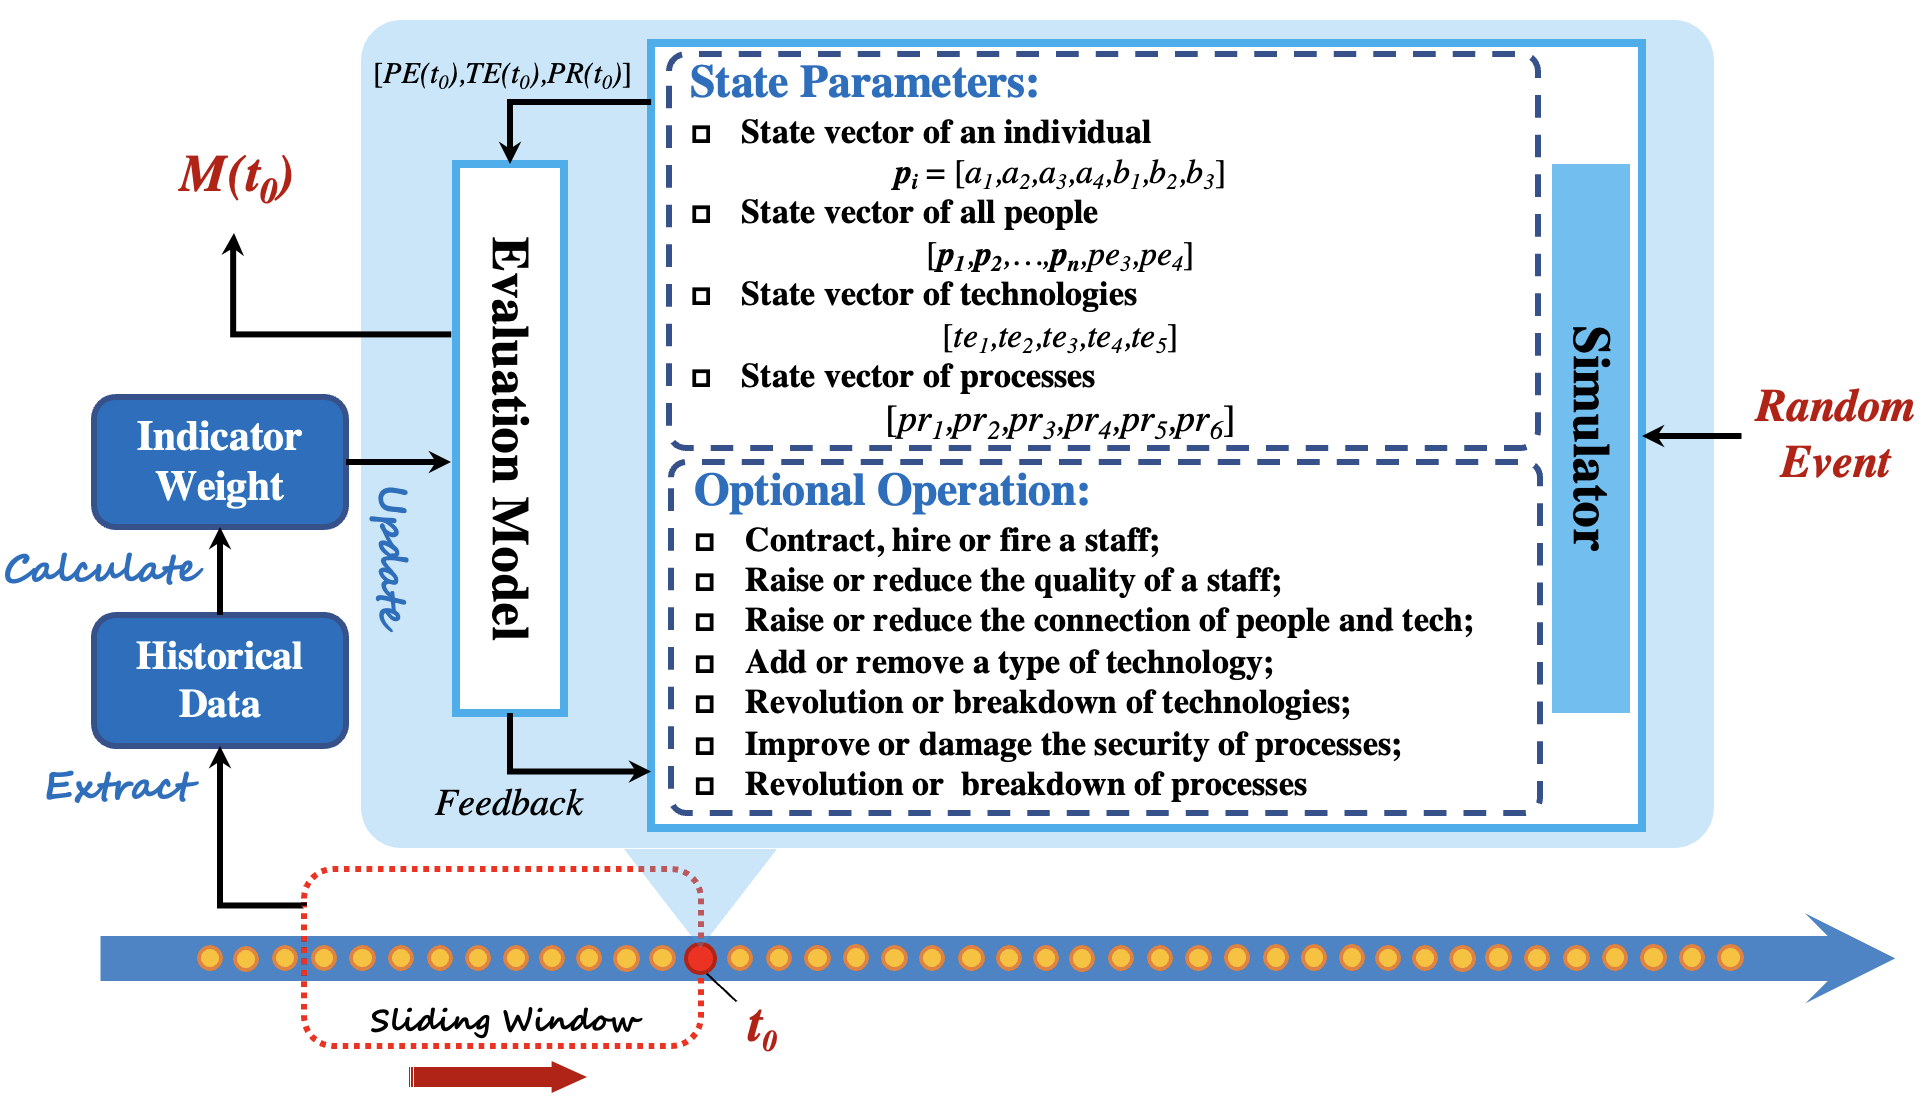
\includegraphics[width=15cm]{figures/simulation.png}
    \caption{Schematic Diagram of Simulation} 
    \label{figure::Schematic Diagram of Simulation}
\end{figure}%figure::Schematic Diagram of Simulation

To simulate the condition of people, we built a pool of candidates, in which an individual is randomly generated with a quality vector
\begin{equation}
    p_i = [a_1,a_2,a_3,a_4,b_1,b_2,b_3]
\end{equation}
and the D\&A system has an state vector 
\begin{equation}
    [p_1,p_2,\dots,p_n,pe_3,pe_4]
\end{equation}
to show how many employees there are, how qualified each employee is and how well they have mastered the technology. The system could hire or fire an employee, improve or reduce the quality of employees, improve or reduce the degree of technical mastery of employees and other operations.

To simulate the condition of technology, we set the state vector $[te_1,te_2,te_3,te_4,te_5]$ at each point. In view of the fact that technological changes rarely appear abrupt changes and generally require gentle and steady growth, we define $M_{TE}(t)$ in accordance with Brownian motion\cite{5}, which means
\begin{equation}
M_{TE}(t+\Delta t)-M_{TE}(t) \sim N(0, \sigma_1^2(\Delta t))
\end{equation}
and the system could perform operations including add or remove a type of technology, revolution or breakdown of technologies and etc..

Like technology, our description of processes is also based on the fact that the process changes in accordance with Brownian motion, which means
\begin{equation}
    M_{PR}(t+\Delta t)-M_{PR}(t) \sim N(0, \sigma_2^2(\Delta t))
\end{equation}
and the system could perform operations including improve or damage the security of processes, revolution or breakdown of processes and etc..

\subsubsection{Operation Process}
At each moment, the system will generate a number of random events, and the simulation system will carry out relevant operations, update the status parameters according to these events. For example, when a random event 'shortage of people' occurs, the system will hire several people from the candidate pool to keep the total number reasonable.

We use sliding window technology to solve the problem of updating the weight of evaluation model. When considering the maturity calculation of $t_0$, we extract the historical data from the pre-set sliding window $[t_0-T_{SPAN},t_0]$, and calculate the model weight according to the PCA method in Section 4. When the next moment is evaluated, the sliding window moves along the timeline to get a new set of historical data. The introduction of sliding window can make the weight of each index of the model more consistent with the current situation, so as to reduce the mutation of the model and improve the accuracy of the model.

\subsection{Optimal Pattern Discovery}
\subsubsection{Optimization Model}
As mentioned in Section 4.5.2 and 4.6.2, the maturity can be evaluated by observing all of the selected indicators, and the optimization is subject to the limited conditions. As there is no such data to build an accurate model to describe this constraint, we assume that the growth of maturity of people, technologies and processes have given upper and lower bounds respectively, and the sum of the growth is limited by a given constant. Therefore, the best pattern to maximize the potential of the data assets could be discovered by solving constrained optimization model shown in Formula \ref{formula::optimization}.
\begin{gather}
    \max M(t) \notag\\
    s.t.\begin{cases}
    L_{M_{PE}} \leq M_{PE} \leq H_{M_{PE}} \\
    L_{M_{TE}} \leq M_{TE} \leq H_{M_{TE}} \\
    L_{M_{PR}} \leq M_{PR} \leq H_{M_{PR}} \\
    \Delta M_{PE} + \Delta M_{TE} + \Delta M_{PR} \leq C
    \end{cases} 
    \label{formula::optimization}
\end{gather}

\subsubsection{Solving Methods}
We use gradient descent strategy to solve this model and provide the solid plan of optimizing the D\&A capabilities.

For the convenience to describe, we note that
\begin{equation}
    M(t) = \mathscr{G}(M_{PE},M_{TE},M_{PR})
\end{equation}
which could be determined by Formula \ref{formula::Mt}. As the gradient descent strategy, moving in the opposite direction of gradient descent will yield the maximum of the function, if any. 

We define $\eta$ as the step size when getting close to the maximum, and as the indicators is impossible to get close to the upper bound and it will be increasingly hard to optimize as the time is going, we define the step size $\eta$ is subject to
\begin{equation}
    \eta^{(k)} = \frac{1}{(1+k)^2}
\end{equation}
as the increase in iterations.

Therefore, with the iterative initial value of $X^{(0)}=(M_{PE}^{(0)},M_{TE}^{(0)},M_{PR}^{(0)})$, the iterative equation\cite{7} can be expressed as
\begin{equation}
    X^{(i+1)} = X^{(i)}+\eta^{(i)} \cdot \nabla \mathscr{G}^{(i)}
\end{equation}
subject to the limitation in Formula \ref{formula::optimization}.

Since the gradient direction represents the direction with the fastest maturity change, the optimal way to improve the maturity of the system is to adjust each index value according to the proportion represented by the gradient. Here, considering the operability in the actual process of the corporation, we suggest the enterprise to adjust in the direction with the largest gradient component among all indicators. And for the convenience of the corporation to use our model, we provide a flow chart as shown in Figure \ref{figure::flowchart}.

\begin{figure}[!htbp]
    \small
    \centering
    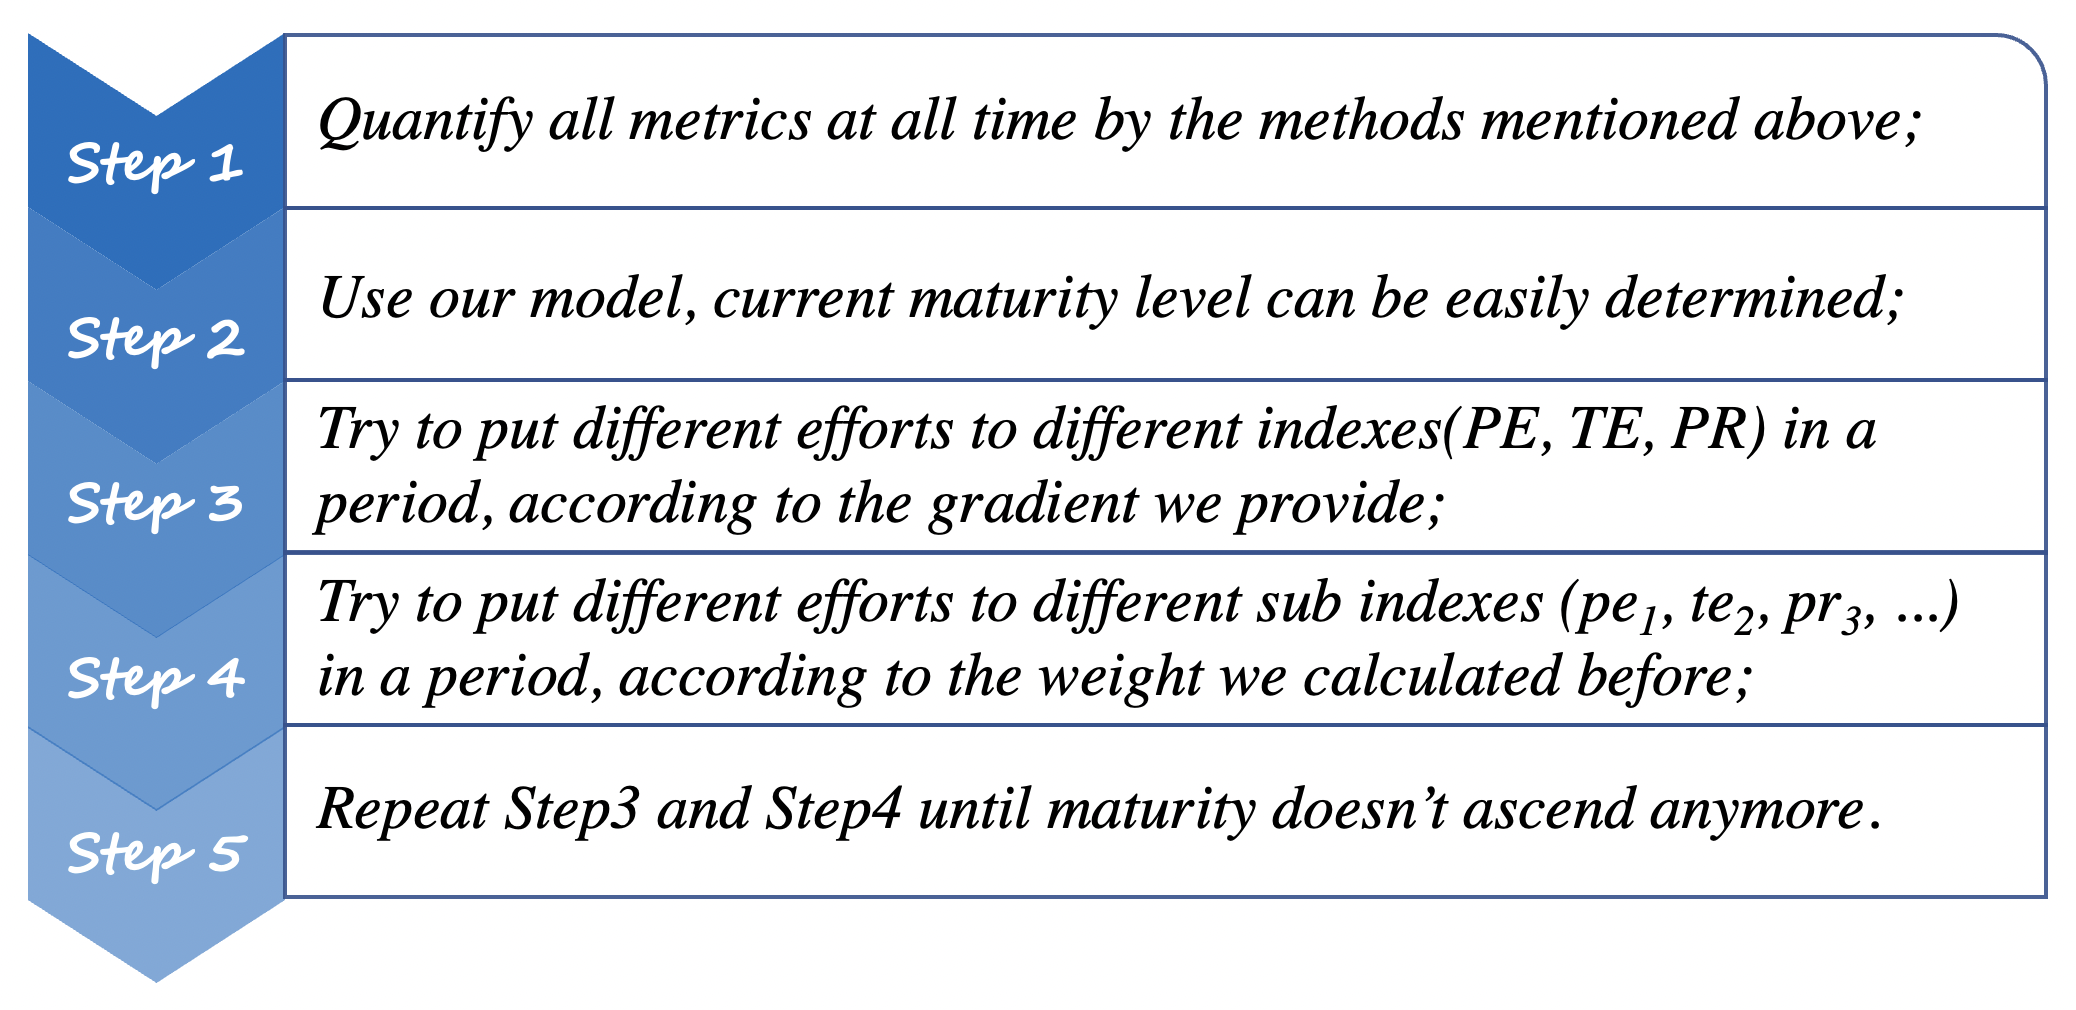
\includegraphics[width=11cm]{figures/FlowChart.png}
    \caption{How to Use Our Model} 
    \label{figure::flowchart}
\end{figure}%figure::flowchart


\subsection{Demonstration on Using the Model}
\subsubsection{Result of Simulation}
We first demonstrate the effect of the simulation system. We consider calculations and assessments on a daily basis over a two-year timeframe. A number of random events are generated at each time node, and the system freely calculates the maturity value at each time point and the changes of each indicator, as shown in Figure \ref{figure::Result of Simulation}.
\begin{figure}[!htbp]
    \small
    \centering
    \begin{tabular}{cc}
        \ 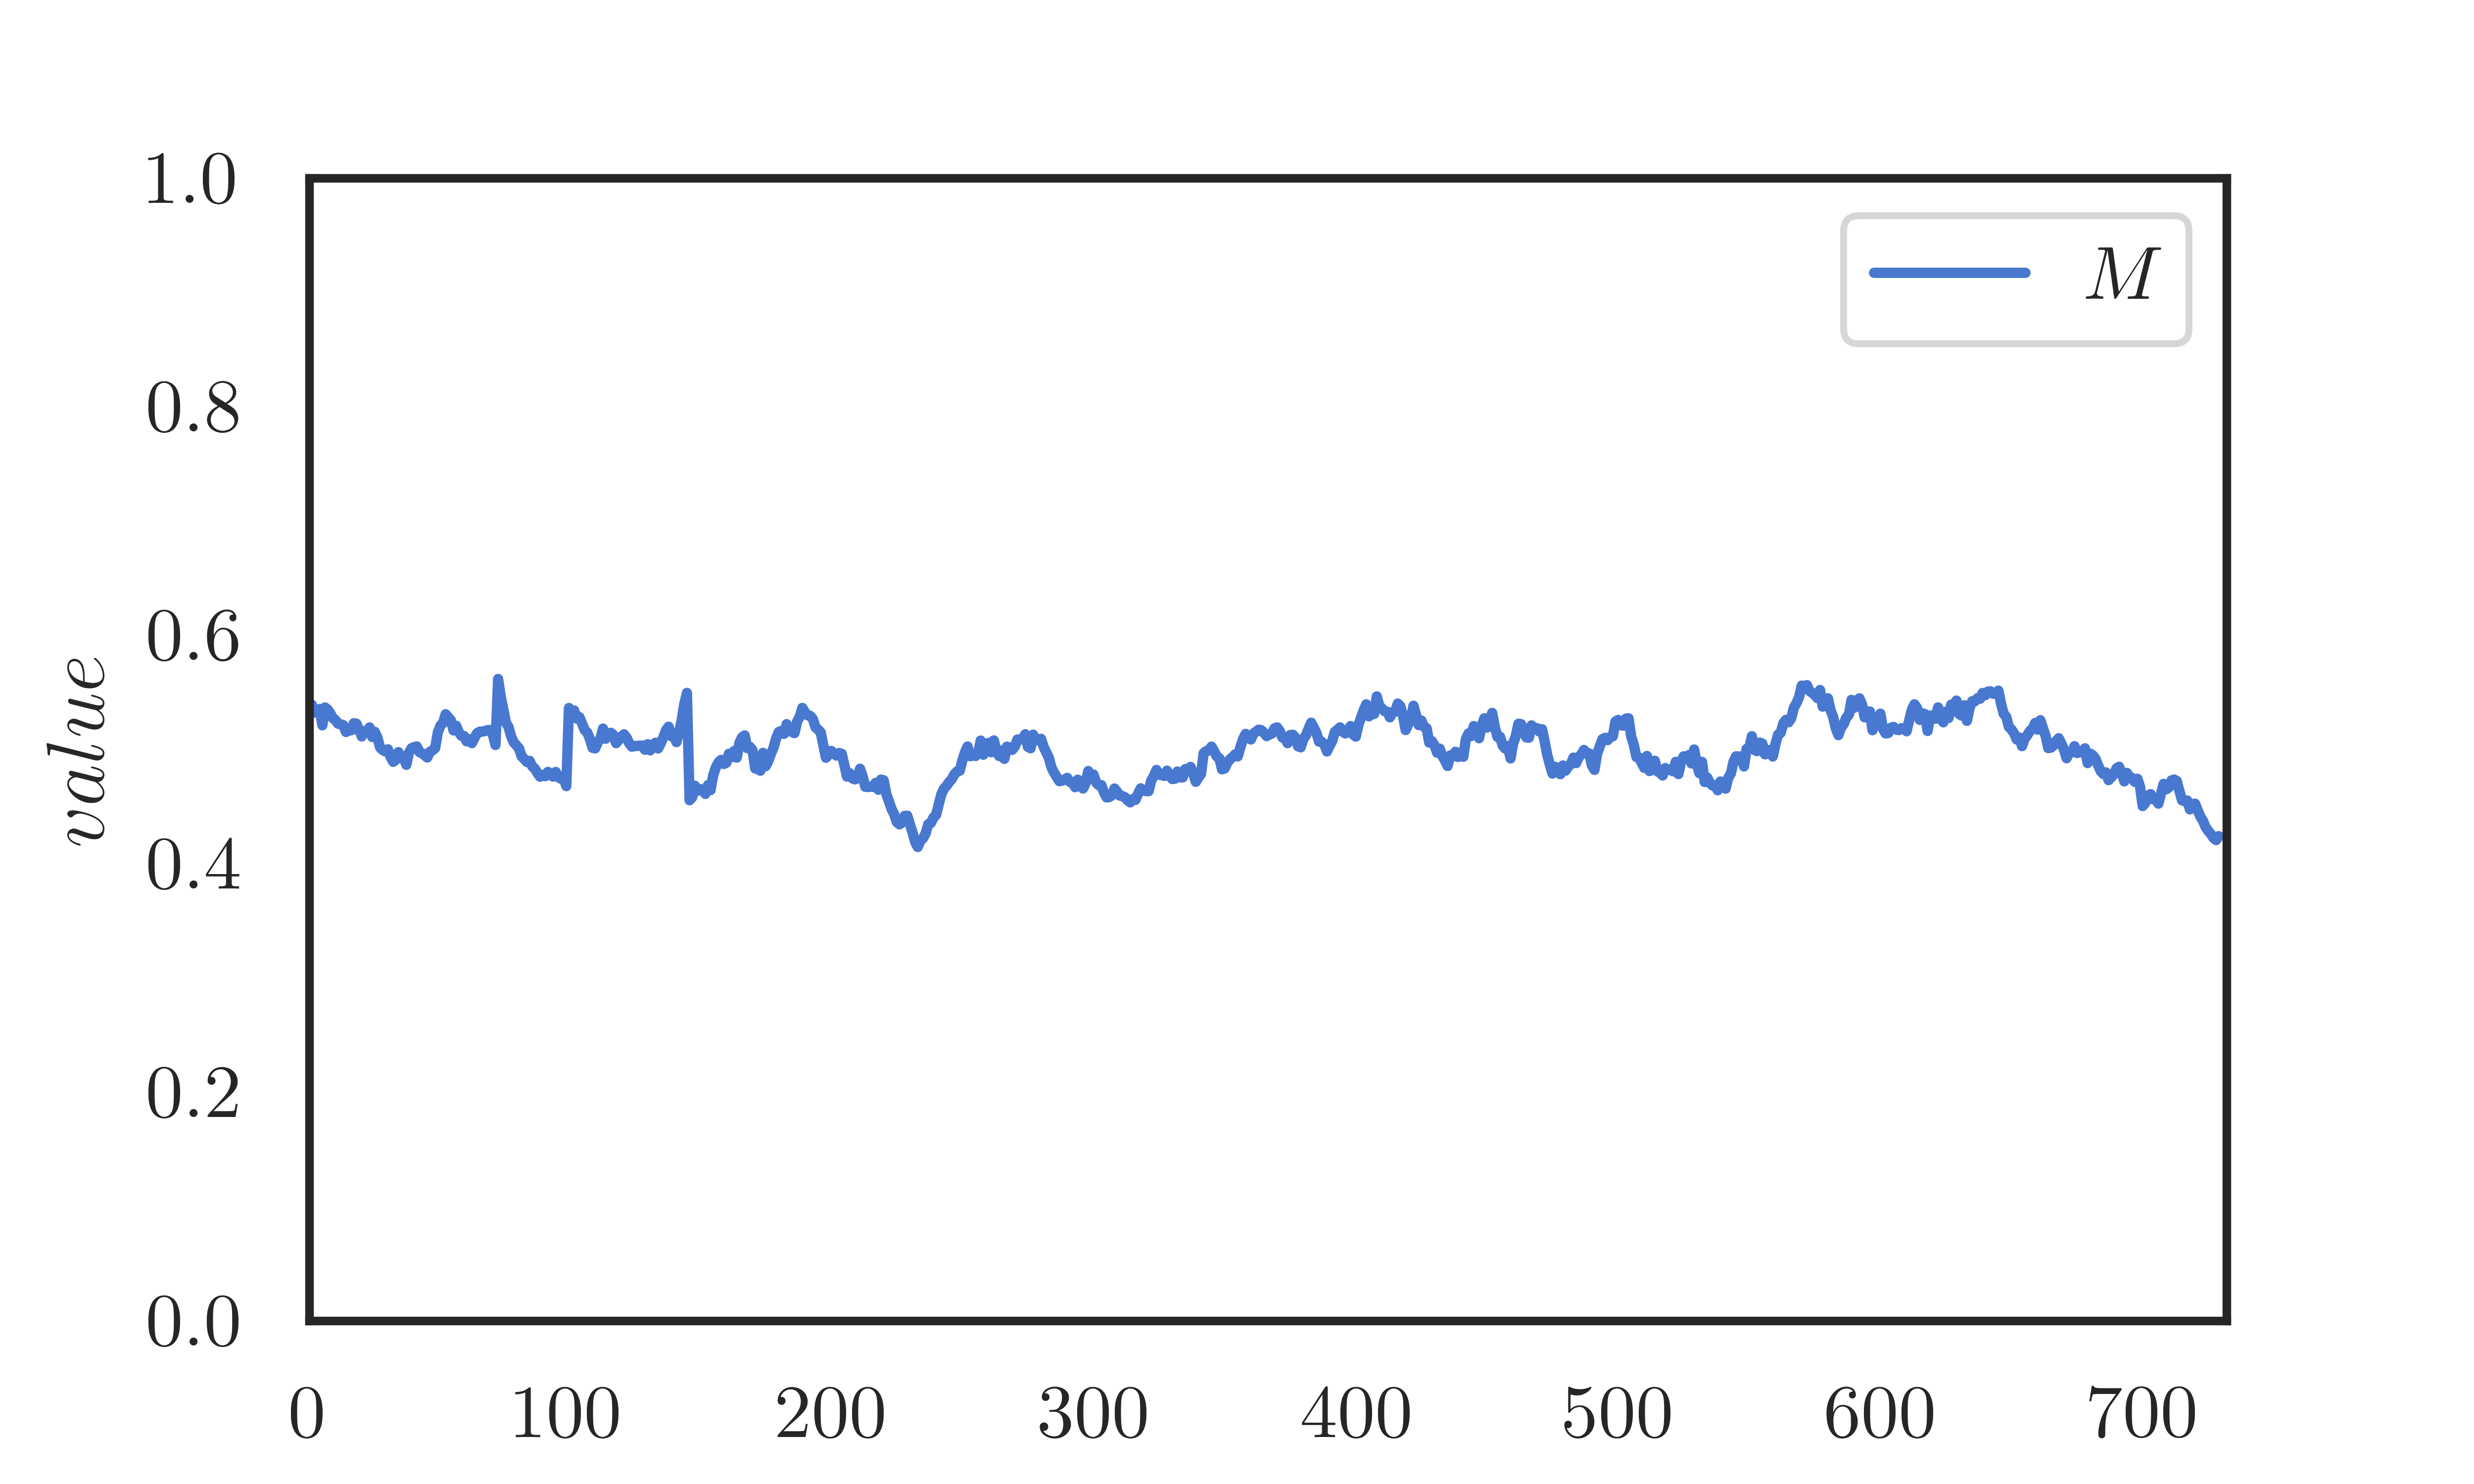
\includegraphics[width=6cm]{figures/simulationresult/M.png} &
        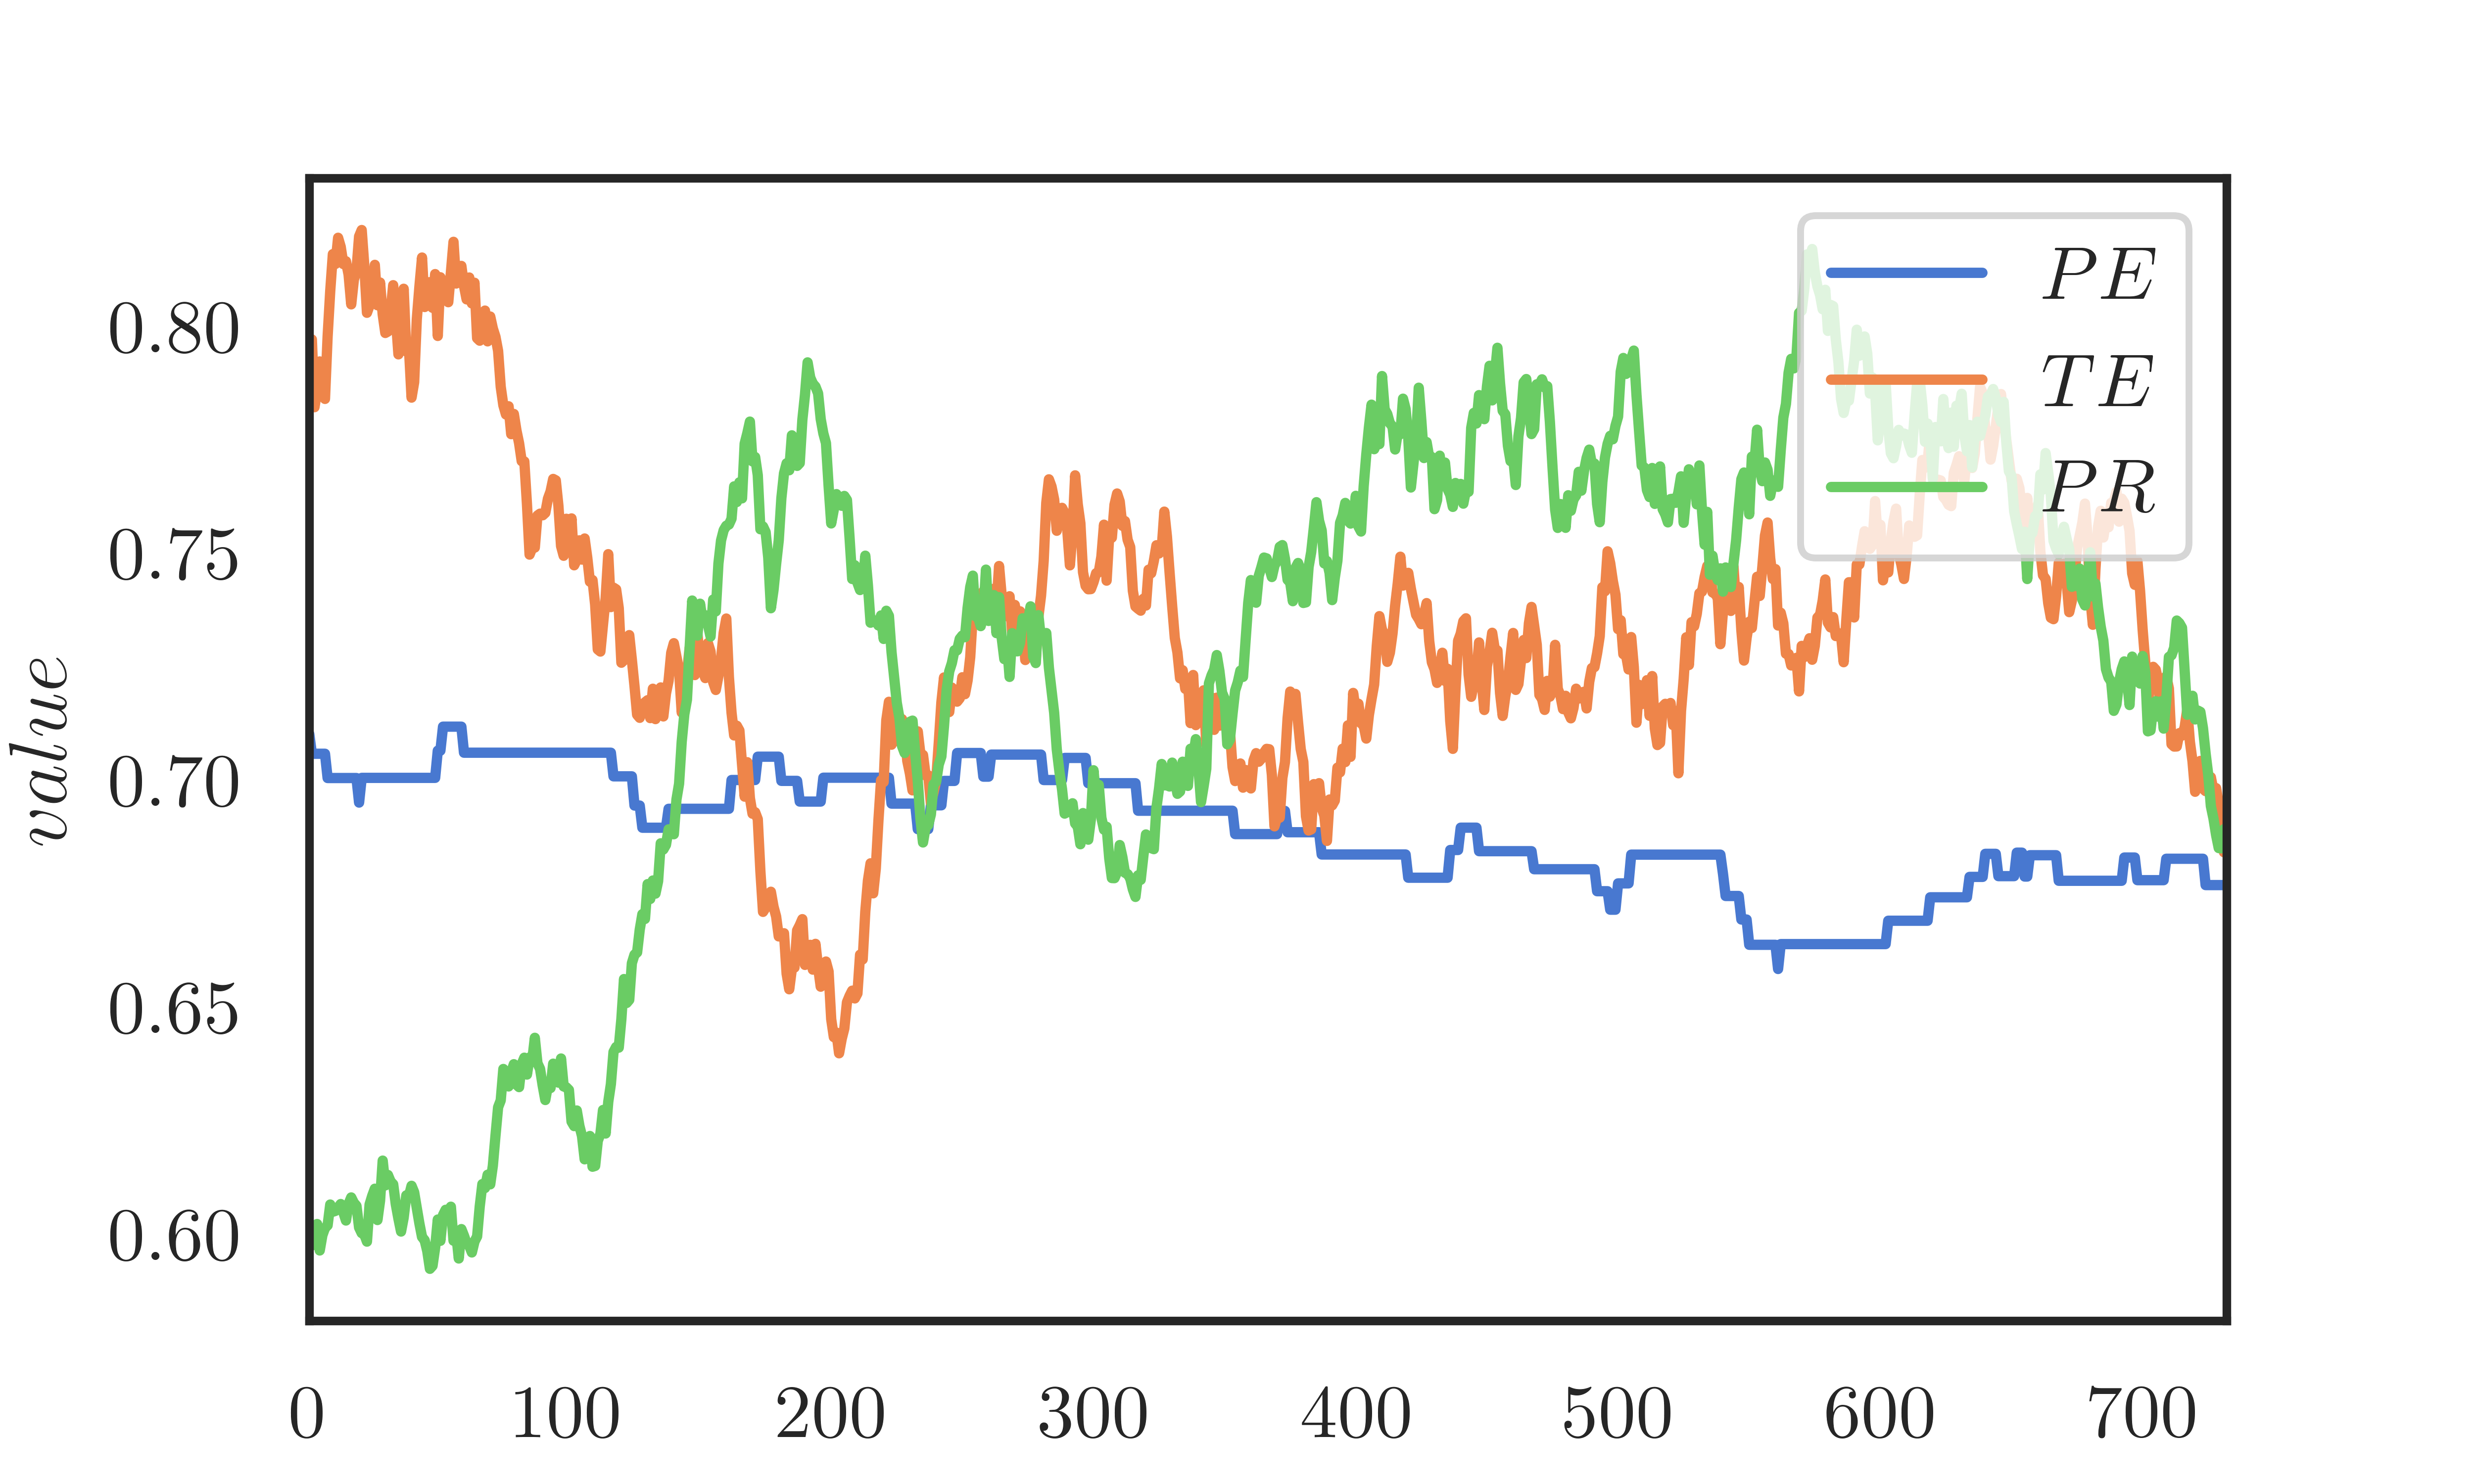
\includegraphics[width=6cm]{figures/simulationresult/inx3_time.png} \\
        $(1)$ & $(2)$ \\
    \end{tabular}
    \caption{Result of Simulation}
    \label{figure::Result of Simulation}
\end{figure}

If the analysis based on the sub-indicators of the model is needed, we can also obtain the change curve of the sub-indicators over time, as shown in Figure \ref{figure::Detailed Result of Simulation}.
\begin{figure}[!htbp]
    \small
    \centering
    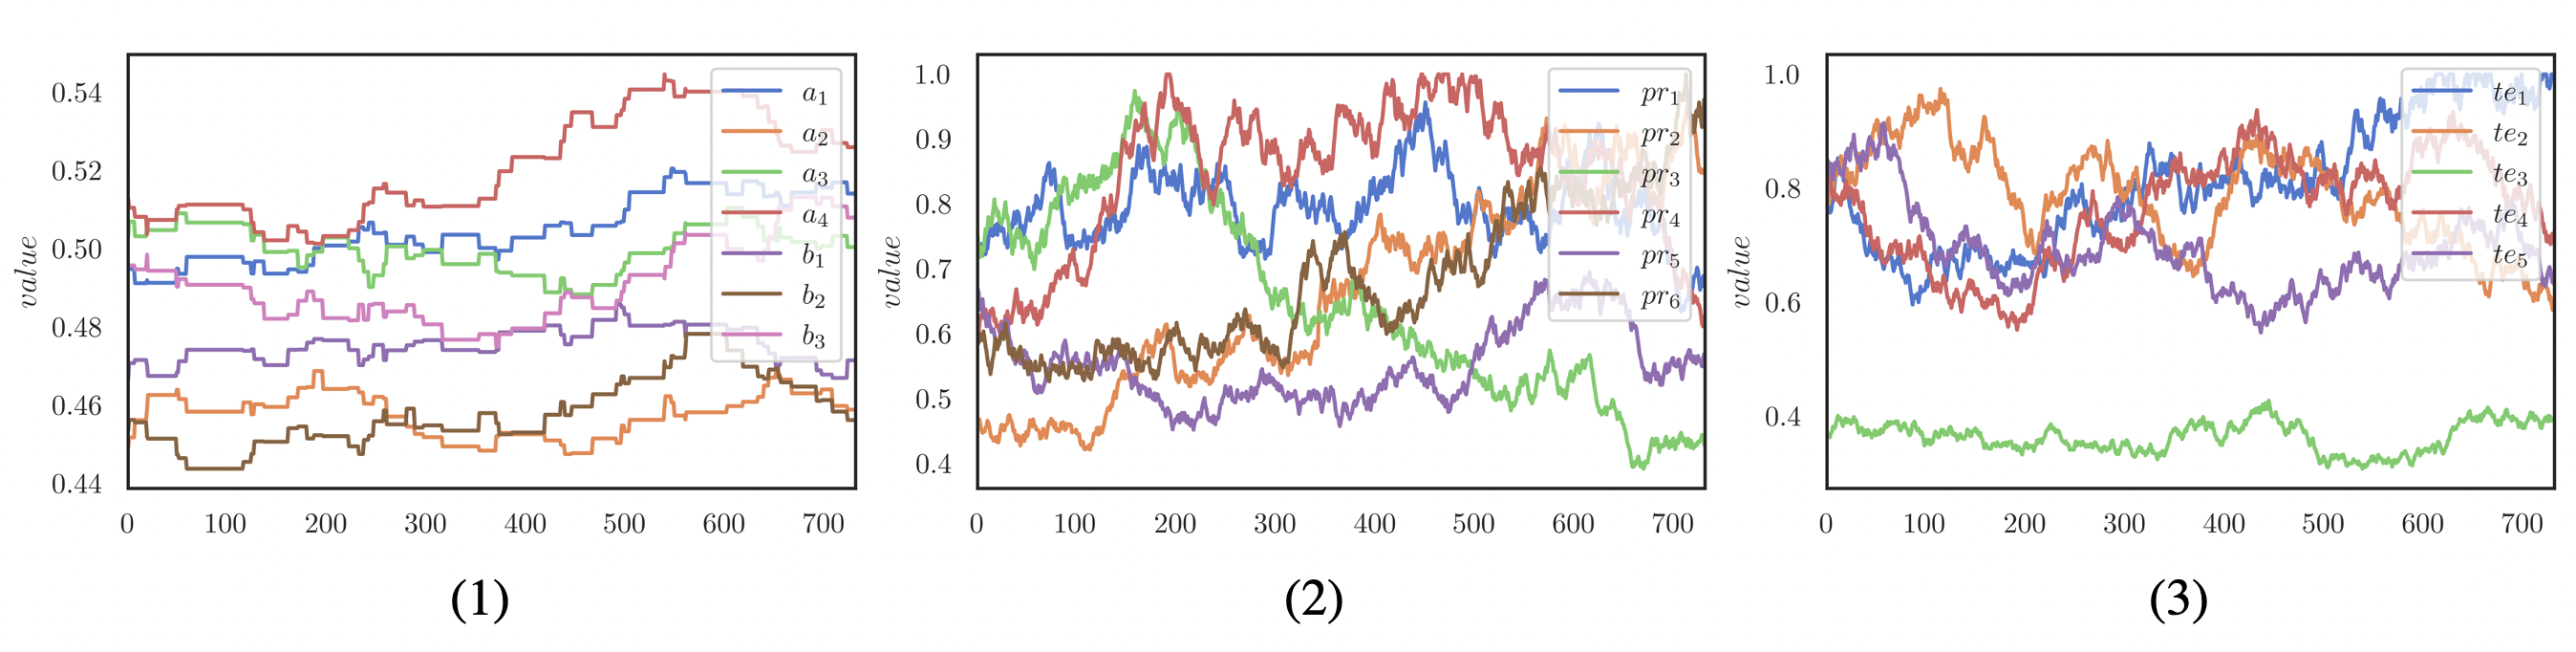
\includegraphics[width=15cm]{figures/simulationresult/petepr.png} 
    \caption{Detailed Result of Simulation}
    \label{figure::Detailed Result of Simulation}
\end{figure}

The simulation results verify the availability of our simulation system. At the same time, according to the figure, while maintaining randomness, the model can also learn strategies that are more conducive to system development based on historical data to ensure the stability of system maturity. This lays the foundation for us to choose the optimal strategy in the next section.

\subsubsection{Result of Optimal Pattern Discovery}
In practice, we adopt two kinds of gradient descent. One of them is mentioned above, another one is to descend in the direction where the component of gradient is largest. From Figure \ref{figure::y3y4}, the blue curves represent the first kind and while orange curves represent the second kind. It can be seen that the blue curve approaches the optimal value faster than the orange one. That's because each step it chooses the optimal direction to descend, and the company can allocate its efforts proportionally according to the gradient to different indexes (people, technologies, and processes). But the orange curve has its own role: the ICM can concentrate only on one main component in one period, which may bring more efficiency.

\begin{figure}[!htbp]
    \small
    \centering
    \begin{tabular}{cc}
        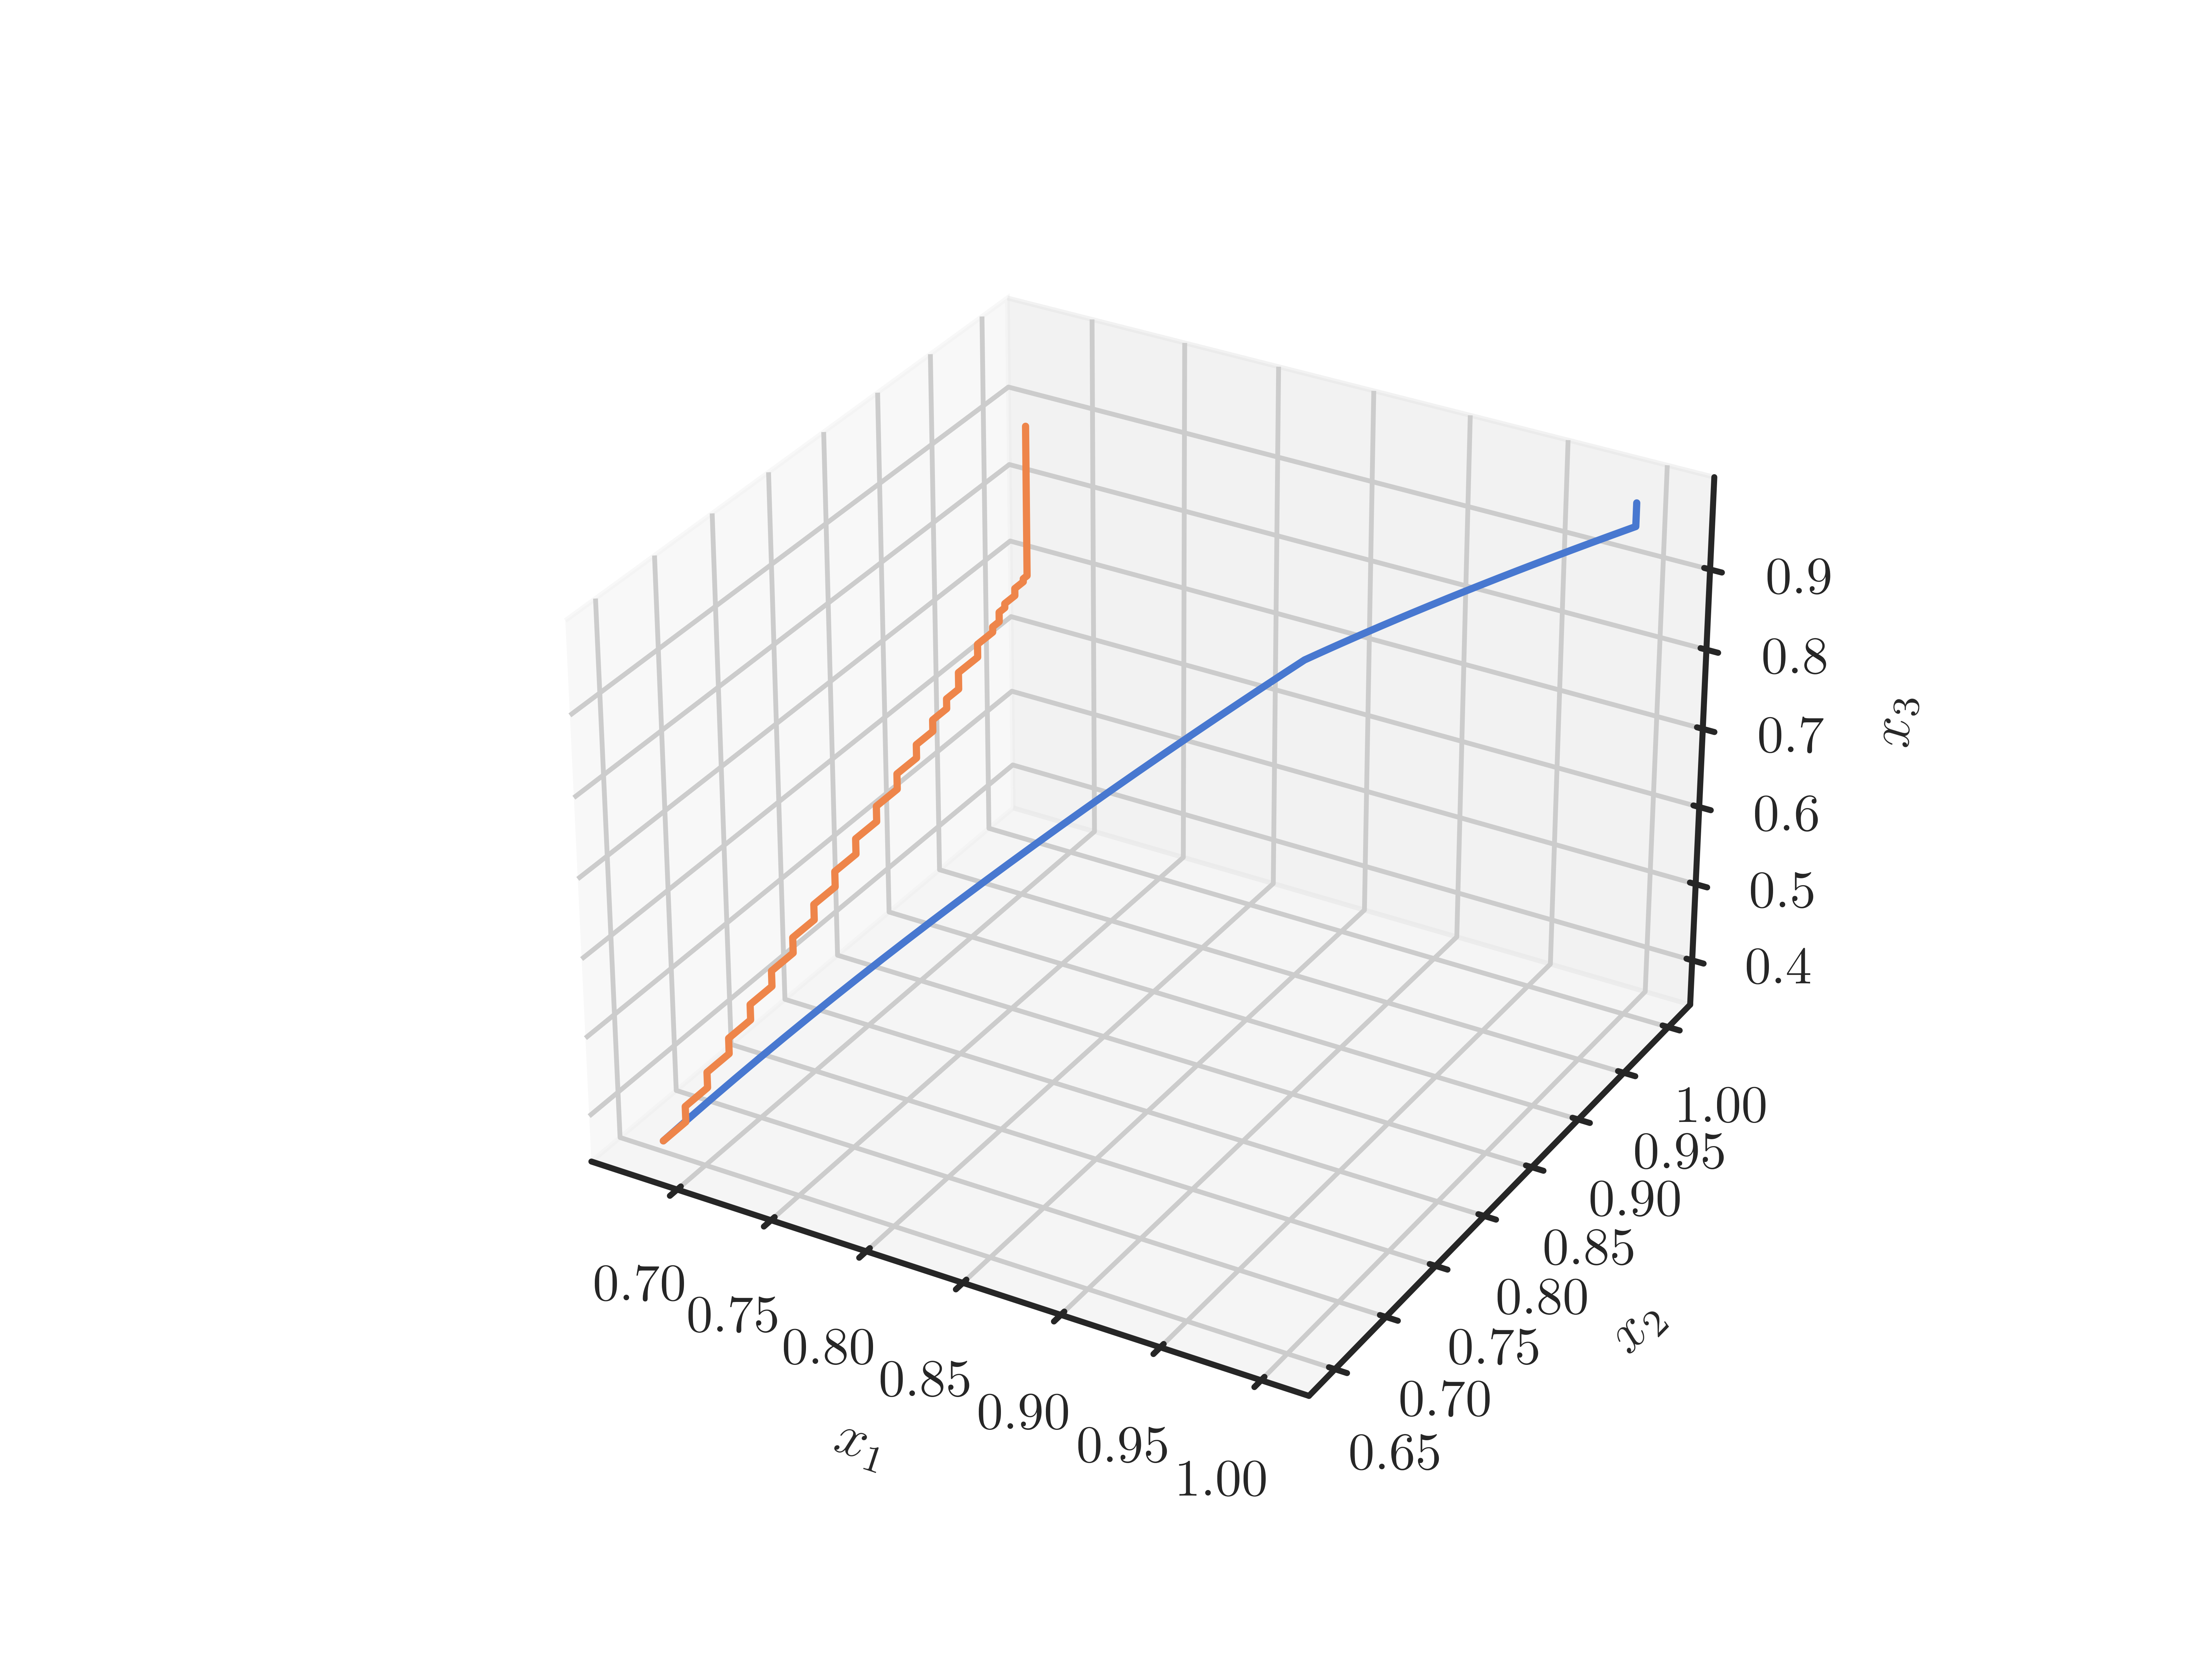
\includegraphics[width=7cm]{figures/21.2.png} &
        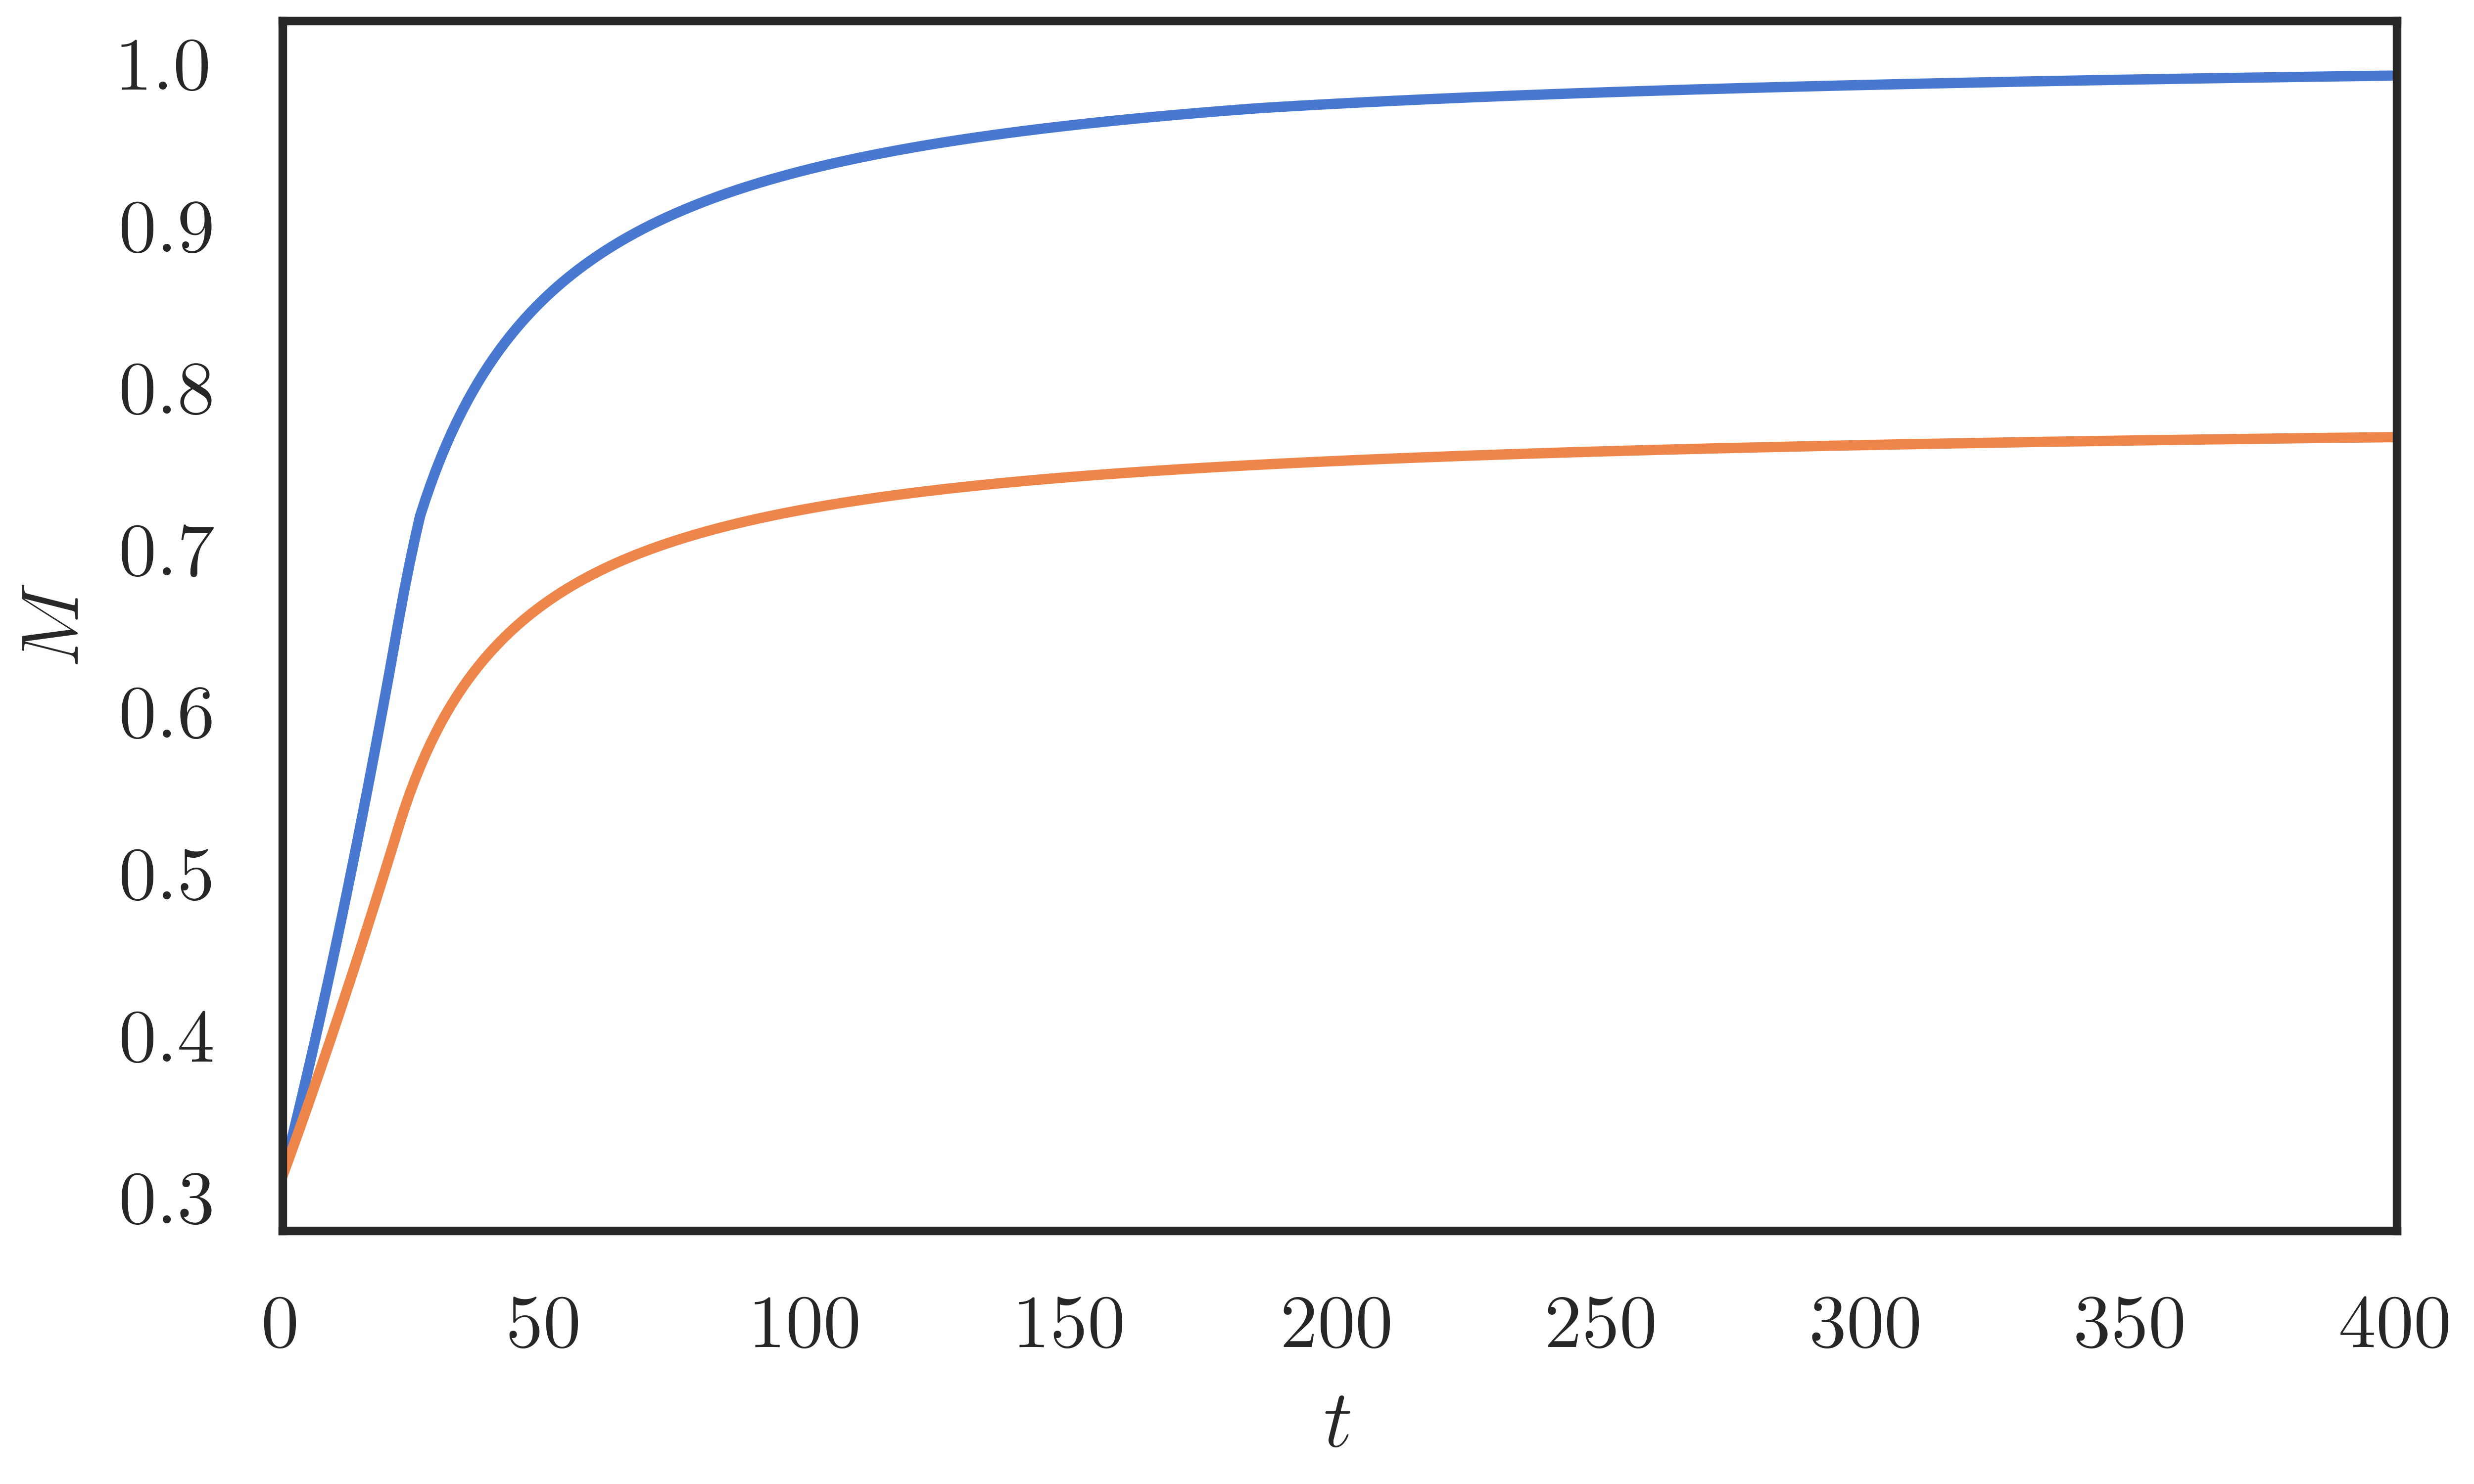
\includegraphics[width=7cm]{figures/y3y4.png} \\
        $(1)$ & $(2)$ \\
    \end{tabular}
    \caption{Result of Optimal Pattern Discovery}
    \label{figure::y3y4}
\end{figure}

\subsubsection{Solid Plan of Optimizing D\&A Capabilities}
Taking the first five steps as an example, Table \ref{table::example} shows what ICM should do in two different algorithms. Each time, ICM should try its best to make its $PE$, $TE$, $PR$ indexes change by $dx_1$, $dx_2$, $dx_3$. Following this solid plan, ICM could increase its maturity gradually.

\begin{table}[!htbp]
    \small
    \setlength{\abovecaptionskip}{0cm}
    \setlength{\belowcaptionskip}{+0.1cm}
    \caption{An Example for the Plan}
    \label{table::example}
    \centering
    \begin{tabular}{ccccccc}  
    \toprule   
    \ & \multicolumn{3}{c}{\textbf{Gradient Descent}} & \multicolumn{3}{c}{\textbf{Modified Gradient Descent}} \\
    \textbf{Step} & $dx_1$ & $dx_2$ & $dx_3$ & $dx_1$ & $dx_2$ & $dx_3$ \\
    \midrule
    1 & 0.0047 & 0.0138 & 0.0137 & 0.0000 & 0.0200 & 0.0000\\
    2 & 0.0048 & 0.0138 & 0.0137 & 0.0000 & 0.0000 & 0.0200\\
    3 & 0.0049 & 0.0137 & 0.0137 & 0.0000 & 0.0200 & 0.0000\\
    4 & 0.0051 & 0.0137 & 0.0136 & 0.0000 & 0.0000 & 0.0200\\
    5 & 0.0052 & 0.0137 & 0.0136 & 0.0000 & 0.0200 & 0.0000\\
    \bottomrule  
    \end{tabular}
\end{table}

%Task 3
\section{\scshape{Task 3:} \upshape{Evaluation of Effectiveness and Protocols}}
In this section, we address the effectiveness assessment of D\&A System and the protocols to measure it. 

We take a comparative approach to evaluation. Firstly, a cargo scheduling optimization model was established to minimize the time of all ships and trains at the port. We design an algorithm to solve the model and get the shortest residence time. We use the residence time and minimum time of the ICM Corporation's current system to construct new indicators as the measurement of the effectiveness of D\&A system.

In the process of solving the optimization model, we can know which index changes can reduce the total residence time and evaluate their impact on the results, based on which we can formulate reasonable protocols to observe and optimize the D\&A system.

\subsection{Evaluation Model of Effectiveness}



\subsubsection{Optimal Cargo Scheduling Model}
We have established a structural model of cargo scheduling at the wharf, as shown in Figure \ref{figure::Cargo Scheduling Model}. In order to simplify the complexity of the analysis, we consider that the dock consists of a ship docking area, a cargo holding area, a train parking area and two transfer equipment. When the ship enters the docking area, the transfer equipment will transport the containers on board to the cargo holding area, if the transfer equipment is idle and there is a vacant position in the cargo holding area. When the receiving train is in position in the train parking area, the transfer unit on the other side loads the containers onto the corresponding train, completing a cargo transfer.
\begin{figure}[!htbp]
    \small
    \centering
    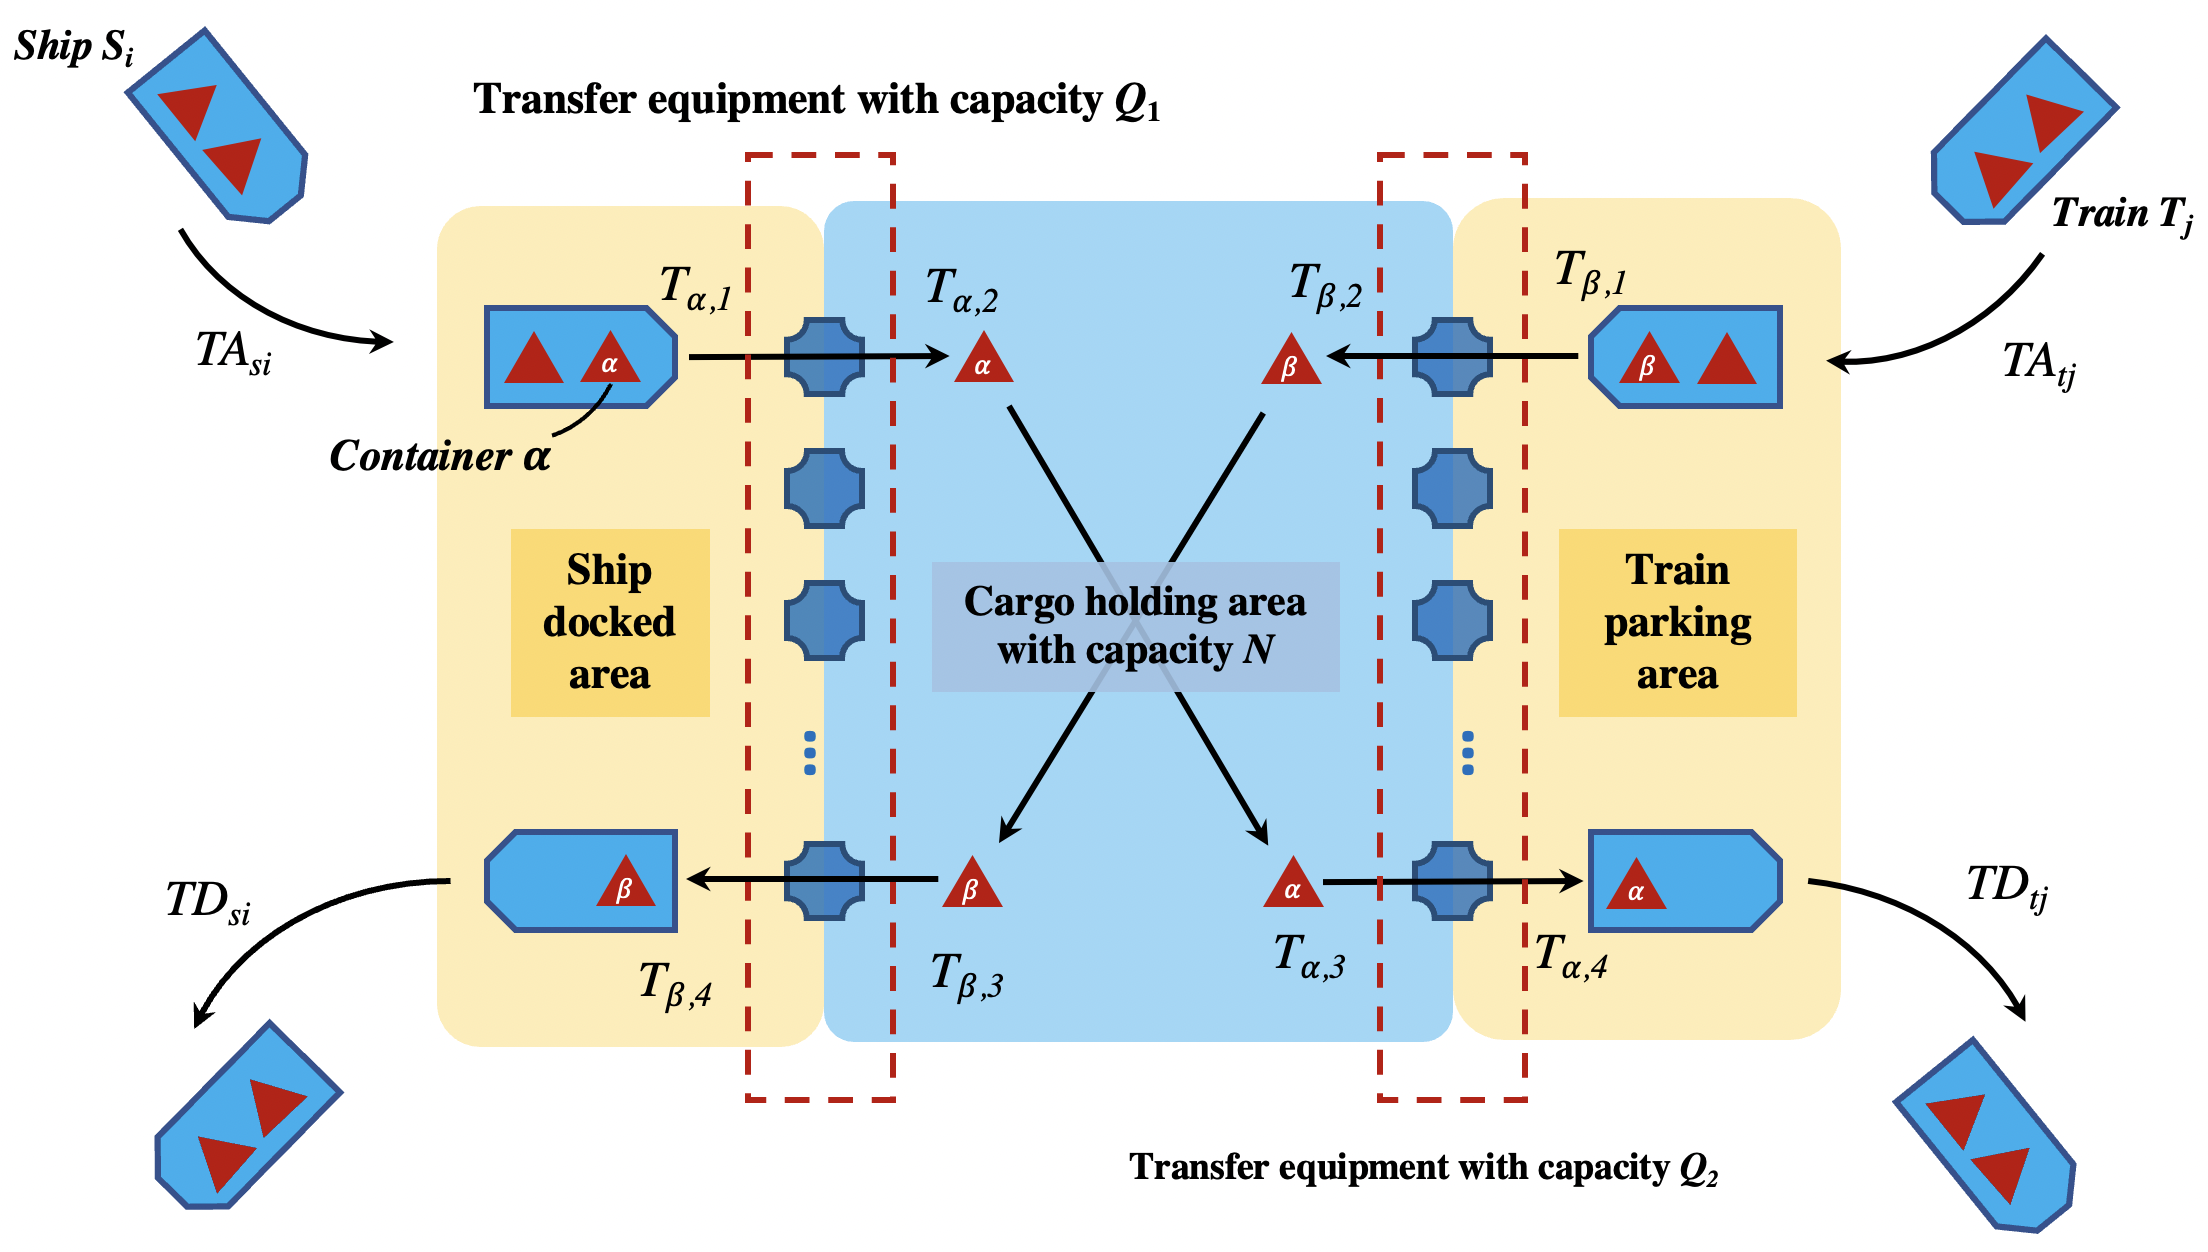
\includegraphics[width=15cm]{figures/DemonstrationonCargoSchedulingModel.png}
    \caption{Cargo Scheduling Model} 
    \label{figure::Cargo Scheduling Model}
\end{figure}%figure::Cargo Scheduling Model

We define the total time of all the ships and trains staying at the port as the optimized objective function within a period of time $T_{span}$ just as
\begin{equation}
    \mathscr{F} = \sum_{i \in I}(TD_{s_i}-TA_{s_i}) + \sum_{j \in J}(TD_{t_j}-TA_{t_j})
\end{equation}
where $TD_{\alpha}$ is the leaving time of vehicle $\alpha$, $TA_{\alpha}$ is the arriving time of vehicle $\alpha$. And the objective function is constrained by several factors.\cite{8}

\textbf{Time constraint from ships to trains.} The transfer of containers follows a time sequence, thus creating a time constraint from one end to the other. We define the time when container $c_{i^{\prime}}$ leaves the ship's docking area, enters the cargo holding area,  leaves the cargo holding area and enters the train parking area respectively as $T_{c_{i^{\prime}},1}$, $T_{c_{i^{\prime}},2}$, $T_{c_{i^{\prime}},3}$, $T_{c_{i^{\prime}},4}$. The time of transportation in transfer equipment is assumed to be $T$ for every container. Therefore, as the time sequence,  the constraint is
\begin{equation}
    \begin{cases}
    T_{c_{i^{\prime}},1} \geq TA_{s_i}, \forall i \in I, \forall i^{\prime} \in S_i\\
    T_{c_{i^{\prime}},2} = T_{c_{i^{\prime}},1}+T\\
    T_{c_{i^{\prime}},3} \geq T_{c_{i^{\prime}},2} \\
    T_{c_{i^{\prime}},4} = T_{c_{i^{\prime}},3}+T\\
    T_{c_{i^{\prime}},4} \leq TD_{t_j}, \mathbf{if}\   \varphi(c_{i^{\prime}},t_j) = 1 
    \end{cases}
\end{equation}

\textbf{Time constraint from trains to ships.} The same as ships to trains, time  from trains to ships follows a time sequence, and the sequence can be defined as 
\begin{equation}
    \begin{cases}
    T_{c_{j^{\prime}},1} \geq TA_{t_i}, \forall j \in J, \forall j^{\prime} \in T_j\\
    T_{c_{j^{\prime}},2} = T_{c_{j^{\prime}},1}+T\\
    T_{c_{j^{\prime}},3} \geq T_{c_{j^{\prime}},2} \\
    T_{c_{j^{\prime}},4} = T_{c_{j^{\prime}},3}+T\\
    T_{c_{j^{\prime}},4} \leq TD_{s_i}, \mathbf{if}\   \varphi(c_{j^{\prime}},s_i) = 1 
    \end{cases}
\end{equation}
where $T_{c_{j^{\prime}},1}$, $T_{c_{j^{\prime}},2}$, $T_{c_{j^{\prime}},3}$, $T_{c_{j^{\prime}},4}$ refer to the time when container $c_{j^{\prime}}$ leaves the train parking area, enters the cargo holding area,  leaves the cargo holding area and enters the ship docking area respectively.

\textbf{Area constraint of cargo holding area.} As our assumption, the cargo holding area has a limited capability $N$ of holding the container. Thus, in any time span, the sum of the containers in cargo holding area is no more than $N$, which could be described, for $\forall t \in T$,as 
\begin{equation}
    \sum_{i^{\prime} \in I^{\prime}} \mathbb{I}(T_{c_{i^{\prime}},2} \leq t \leq T_{c_{i^{\prime}},3}) + \sum_{j^{\prime} \in J^{\prime}} \mathbb{I}(T_{c_{j^{\prime}},2} \leq t \leq T_{c_{j^{\prime}},3}) \leq N
\end{equation}
where
\begin{equation}
    \mathbb{I}(X) = \begin{cases}
        1, when \ X \ is \ true;\\
        0, else.
    \end{cases}
\end{equation}

\textbf{Capability constraint of transfer equipment.} In reality, the transfer capacity of one transfer equipment is limited, so we set the upper limit $Q_1$ or $Q_2$ for each transfer machine, so for $\forall t \in T$, the capability constraint can be described as
\begin{equation}
    \begin{cases}
    \sum_{i^{\prime} \in I^{\prime}} \mathbb{I}(T_{c_{i^{\prime}},1} \leq t < T_{c_{i^{\prime}},2}) \leq Q_1 \\
    \sum_{j^{\prime} \in J^{\prime}} \mathbb{I}(T_{c_{j^{\prime}},1} \leq t < T_{c_{j^{\prime}},2}) \leq Q_2
    \end{cases}
\end{equation}

\textbf{Order constraint of containers.} Actually, in a ship or a train, the loading or unloading  of the container has a definite order. As we define the id of each container following this order,  we add the order constraint of containers as 
\begin{equation}
    \begin{cases}
    T_{c_{i_1^{\prime}},1} < T_{c_{i_2^{\prime}},1}, \forall \  i_1^{\prime},i_2^{\prime} \in s_i, i_1^{\prime}<i_2^{\prime} \\
    T_{c_{j_1^{\prime}},1} < T_{c_{j_2^{\prime}},1}, \forall \  i_j^{\prime},j_2^{\prime} \in t_j, i_j^{\prime}<j_2^{\prime}
    \end{cases}
\end{equation}

Up to now, we have built the optimal cargo scheduling model to calculate the shortest time of residence. This will be used to measure the effectiveness in the next section.

\subsubsection{Algorithm to Solve the Model}
We designed a scheduling algorithm based on time series analysis and greedy strategy to solve this model, and the specific process is shown in Appendix A by pseudocode.



\subsubsection{Effectiveness of the System}
By solving the model in section 6.2.1, we can get the minimal sum of time of residence.  With a strategy of comparison, we define the effectiveness of ICM Corporation's D\&A system in the time period of $(i,j)$  as 
\begin{equation}
    EFF(i,j)=\frac{T_E}{T_R}, T_R>T_E
\end{equation}
where $T_E$ denotes the theoretical minimal sum of time and $T_R$ denotes the real sum of time. It is believed that our solution is close to optimal, thus the $EFF(i,j)$ is always no more than 1.


\subsection{Protocols to Measure the Effectiveness}

\subsubsection{Use Standard}
In a period, if the number of ships and trains coming is too small or too large, the protocols cannot be used.

The data of the system needs to be maintained every day. If there's some errors, report. 

\subsubsection{Operating Procedures}
\textbf{Data Collecting}

Collect data in a period(an hour, a day, or a week) which is interesting from database, by selecting the start point and the end point.

\textbf{Data Preprocessing.}

Check if there's any missing data. If yes, operate it according to its number of missing data; if there's a lot of missing data, terminate it and report error; else, select a proper method to fill the missing value, such as CART, filling with average, filling with neighbor, etc. If not, calculate the real sum of waiting time according to data.

\textbf{Applicate the Model to Calculate and Judge the Effectiveness}

Use our model and algorithm on the data extracted to calculate the sum of waiting time.


%Task 4
\section{\scshape{Task 4:} \upshape{Extention of the Model}}

\subsection{Demonstration for Applying the Model to Seaport in Different Scales}
In the seaport model constructed above, there are 3 main indicators to decide the scale of a seaport, $Q_1$, $Q_2$, $N$. Let's consider the operation in different levels of $Q_1$, $Q_2$, $N$. To be real, we assume that time interval between ships/trucks/trains arriving at the port is independent of each other and obeys Poisson distribution whose strength is $\lambda$. Set the inspected period to be $(0,24)$, $T=1$, the average number of containers in a ship $n=5$. Test each case 100 times, and calculate the average. From the table, it can be seen that as the scale gets larger, the sum of waiting time is increasing at almost a square speed. However, our greedy algorithm performs better than random algorithm obviously, especially on a larger scale.

\begin{table}[!htbp]
    \small
    \setlength{\abovecaptionskip}{0cm}
    \setlength{\belowcaptionskip}{+0.1cm}
    \centering
    \caption{Result of Evaluation}
    \begin{tabular}{cccc}  
    \toprule   
    \  & \textbf{Smaller Seaport} & \textbf{General Seaport} & \textbf{Bigger Seaport}\\
    \midrule
    \tabincell{c}{\textbf{Properties}\\$[Q_1,Q_2,N,\lambda]$} &  $[5,5,100,1]$ & $[50,50,1000,10]$ & $[500,500,10000,100]$\\
    \tabincell{c}{\textbf{Sum of waiting time}\\(Greedy algorithm)} & 1157.27 & 105866.17 & 9687230.68\\
    \tabincell{c}{\textbf{Sum of waiting time}\\(Random algorithm)} & 1165.43 & 125056.90 & 15693369.89\\
    \bottomrule  
    \end{tabular}
\end{table}

\subsection{Analyze Adaptation of Maturity Metric to Other Industries}
\subsubsection{General Analysis}
In the model of judging the D\&A system maturity, we mainly considered the influence of people, technology and process, each represented by indexes $PE$, $TE$, $PR$. If all of the three indexes can work well, we can say the maturity metric also works. So let's examine them respectively.

\textbf{PE}. In most situations, an industry needs people as manual workers or mental workers. If there are people, then the index $PE$ works. Because if there are people, their quality indexes and performance indexes can be quantified by means we mentined before, then $PE$ works. Failing situations include but are not limited to: a high-tech company whose labor is all robots, a backward industry which uses animals as labor.

\textbf{TE}. Technology is the driving force for the progress of human society, and many companies value technologies very much. So it is concluded that, similar to $PE$, in most situations $TE$ works. In most sense, if technologies exist, there are always means to assess the 5 different sub indexes, so $TE$ can be calculated and be used to evaluate the excellence of the technology. Here's one situation where $TE$ may not work: in some newly emerging industries where there is only one kind of technology that sub-index Industry Leading Degree can't be assessed, $TE$ fails.

\textbf{PR}. A good governance program provides a lot of convenience and profit. In most sense, as long as an enterprise is running, it has its unique processes which can be assessed in 6 different sub indexes. Then, the index $PR$ works, and can be used to measure the excellence of processes. A possible situation where $PR$ fails is listed here: an enterprise is about to go out of business and all processes are forced to be abandoned.

According to analysis above, to draw a coclusion: in most situations our maturity metric can be adapted to other industries easily. But note that the weights of each index and sub-index are obtained according to the relative importance of each index and the properties of different samples. So when applying the maturity metric to different industries and different companies, it is necessary to recalculate the weights of each index according to the actual situation, and flexibly adjust the models we have established instead of completely copying them. And in a few special situations, maturity metric doesn't work, but it's important to examine each (sub) index.

\subsubsection{Example}
A truck transportation company can also use our indicators. However, as mentioned earlier, some adjustments need to be made to the model.

\textbf{Differences}. Obviously, the requirements for employees are obviously different from those of a truck transportation company. ICM Corporation operates a large seaport, and the people it hires need to have a certain understanding of all matters related to port operation. Truck transportation company drivers need more skilled vehicle driving skills, while port workers may need more skills in driving ships and cranes. Such differences also exist in technical indicators as well as process indicators. 

\textbf{Solutions}. A docker from ICM Corporation and a driver from a truck transportation company have a lot in common. As long as people, technology and processes are mapped one by one, the evaluation of the model will not have much difference. Therefore, after we flexibly adjust the evaluation criteria of the model, we can still get an objective, scientific and reasonable evaluation by the methods described previously.

\subsection{ICM Corporation's Benefits from the Promotion of Indicators}
When truck transportation companies also adopt our indicators, there are many benefits for ICM Corporation as follows,

\textbf{Improving the system.} When truck transportation companies use our indicators, they may find some defects that ICM Corporation is not aware of. In this way, we can timely revise and supplement our indicators and avoid greater losses to ICM Corporation in the future. Besides, more data means more assets. Mining in a bigger dataset may generate more accurate and interesting patterns, which can also provide help for improving the system.

\textbf{Building confidence.} Only reliable and practical systems will be more widely used. Other companies use our indicators, which further proves the rationality of the indicators from the side. And ICM Corporation's social influence and popularity have been further improved.

\textbf{Generate revenue.} This interaction with other companies also has implicit benefits. It helps ICM Corporation expand its business and make more profits in the future. Besides, our system can improve the transportation efficiency of the truck transportation company, which helps to reduce the detention time of goods in the port, and improve the efficiency of cargo transportation.

%Final Remark
\section{Final Remark}
In this section, we'll make a general summary of our work, including the model we built, the results we found, the suggestions we provided, the pros \& cons of our methods, and the future development of our model.

\subsection{Sensitive Analysis}
Now, we consider the influence of parameters on the index score under different fluctuation states. As shown in Figure \ref{figure::sen1}, the greater the parameter fluctuation, the greater the score fluctuation
\begin{figure}[!htbp]
    \small
    \centering
    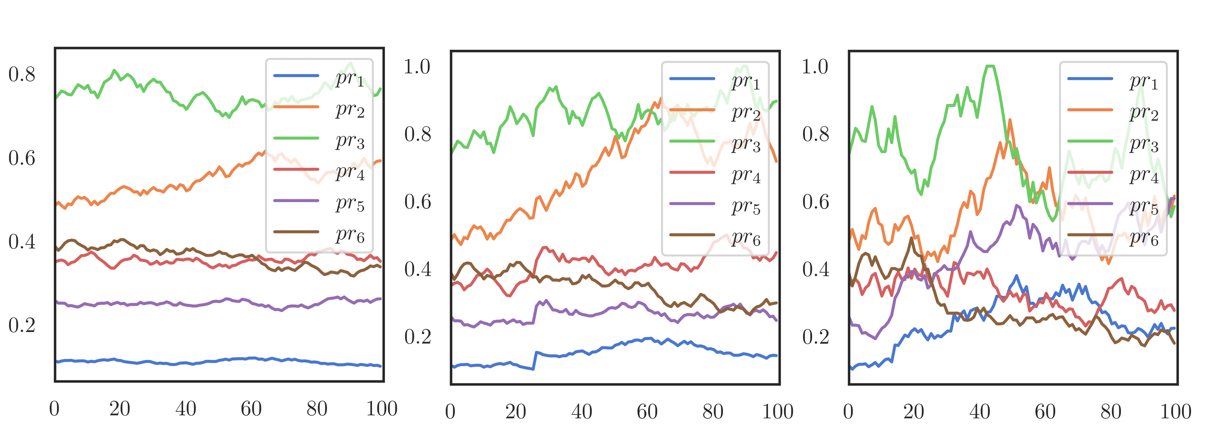
\includegraphics[width=13cm]{figures/sen1.png}
    \caption{Sensitive Analysis for Model 1} 
    \label{figure::sen1}
\end{figure}

To make a solid plan for ICM, we use gradient descent measure to approach the optimal value. To consider the effect of step size, we choose different step sizes and quantitatively analyze the maturity change of the system. In Figure \ref{figure::sen2}, the first graph adopts constant step size, and the remaining two graphs adopt different variable step size respectively. The three axes are people, technologies and processes. The first figure represents that in the ideal state, with the growth of three indicators, the maturity of the system gradually approaches 1. However, it is impossible for the system maturity to reach 1 in practice. The remaining two figures well reveal that the system maturity will reach a limit value in practice.
\begin{figure}[!htbp]
    \small
    \centering
    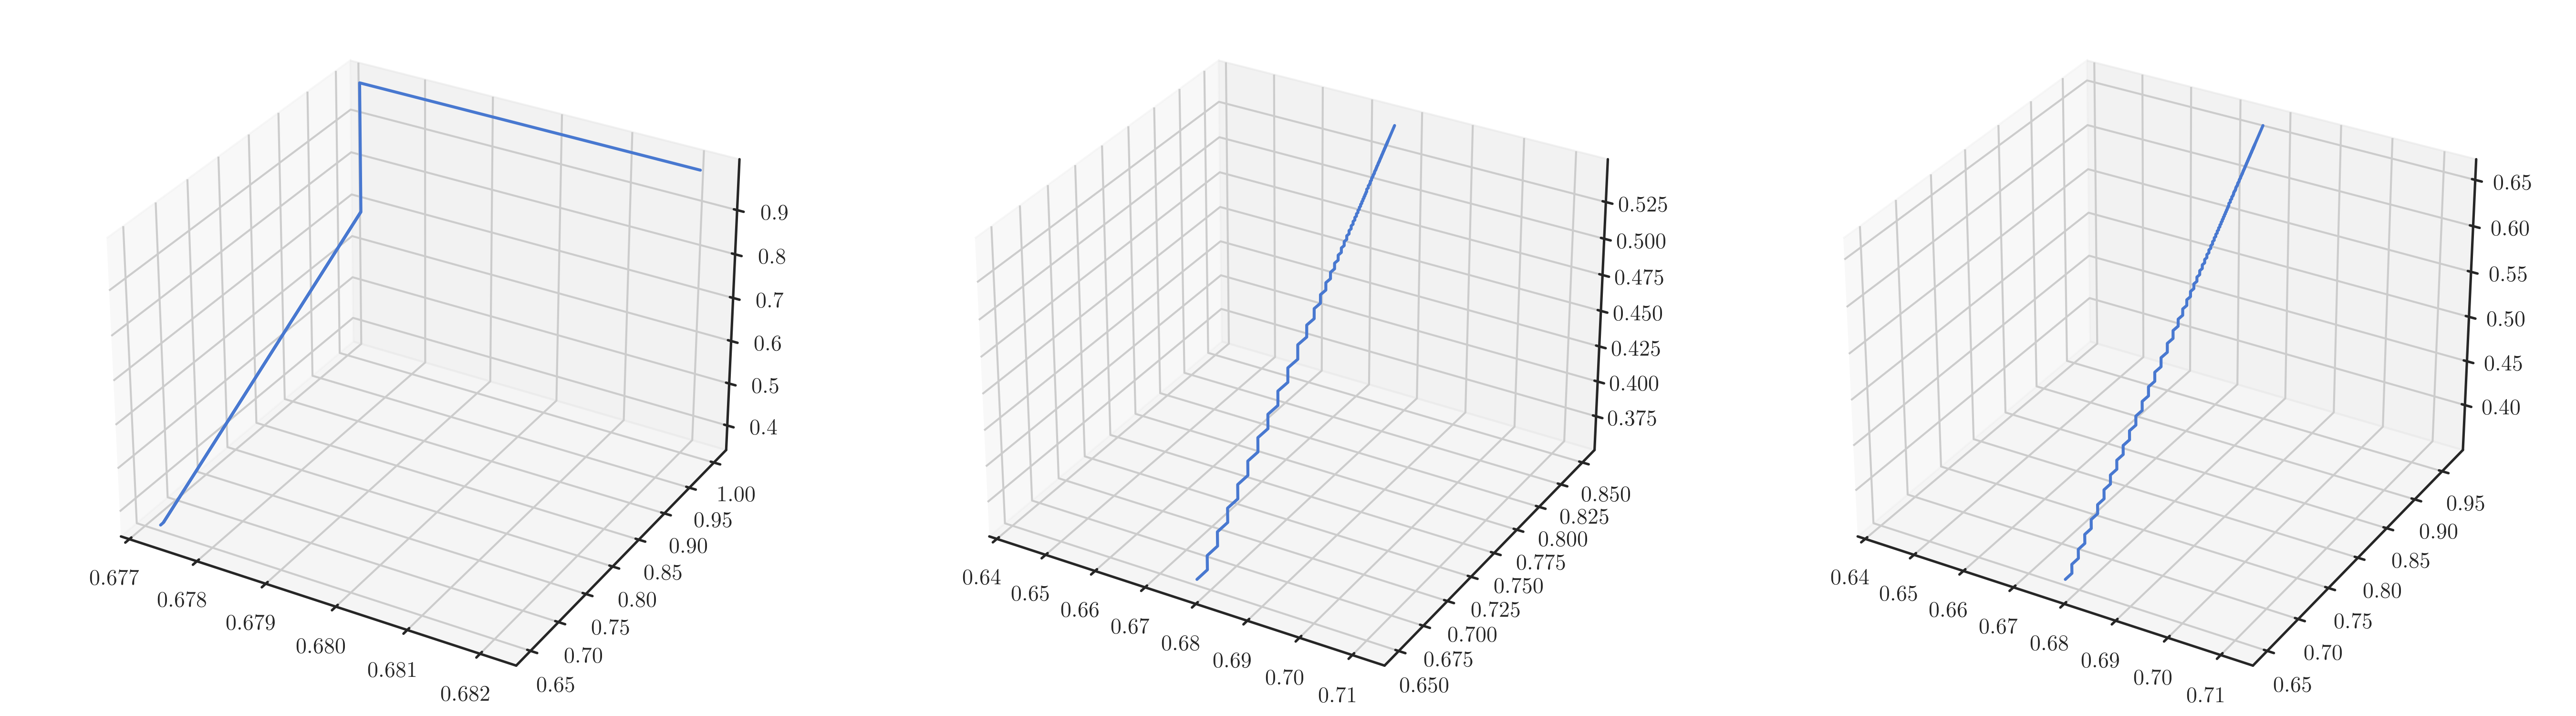
\includegraphics[width=15cm]{figures/sen2.png}
    \caption{Sensitive Analysis for Model 2} 
    \label{figure::sen2}
\end{figure}

\subsection{Strengths and Weaknesses}

\subsubsection{Strengths}
\begin{itemize}
    \item \textbf{Mechanism based construction. } By analyzing the internal composition and connection of the system, we set up an evaluation model of the maturity and effectiveness of the system, and give a concrete demonstration to verify its feasibility, which is highly interpretable.
    \item \textbf{Easy to learn and operate.} The index system selected by the model is easy to obtain in daily operation or from the test. The model provides a complete use scheme and evaluation strategy, which is easy for the corporation to understand and apply.
    \item \textbf{Strong generalization ability.}  For the maturity evaluation model, the parameters themselves are suitable for the evaluation of various systems; for the cargo scheduling model, the parameters of the model can be well extended to more general conditions, so as to be applicable to the evaluation of more scheduling systems.
\end{itemize}

\subsubsection{Weaknesses}
\begin{itemize}
    \item \textbf{Lack of real data to test and verify.}  As for evaluation models, data-based models tend to reflect reality better, while mechanism-based models pay more attention to theoretical analysis, which is sometimes inaccurate. Only when there is enough data for analysis can the parameters of the model be determined more accurately, and then more accurate evaluation can be carried out.
    \item \textbf{Simplified evaluation index system.}  In reality, there are too many indicators reflecting the maturity and effectiveness of the system, and we only extract the main influencing factors to build the model. Therefore, it is inevitable to ignore some potentially valuable information.
\end{itemize}

\subsection{Future Work}
\begin{itemize}
    \item \textbf{Improve the model based on data.}  If we can get more realistic data, we can adopt more realistic methods, such as machine learning, to modify our model or optimize the parameters of the model, so that the calculation results of the model have more realistic effects.
    \item \textbf{A more detailed evaluation system.}  If we can have a better understanding of ICM Corporation's business, operation mode and demand, we can refine and improve the existing evaluation index system, so that it can meet the real requirement  better and achieve better evaluation results.
    \item \textbf{More specific protocols and measures.}  Due to the lack of understanding of the current rules and requirements of ICM Corporation, our protocol is proposed from an idealized perspective, which can be refined and improved in the future according to reality.
\end{itemize}




%Reference
\newpage
\begin{thebibliography}{99}
\bibitem{1}Fanderl H, Stone D, Pulido A. Don't Let Data Paralysis Stand Between You and Your Customers. 
%EWM
\bibitem{2}Mon, D. L. . (1995). Evaluating weapon system using fuzzy analytic hierarchy process based on entropy weight. IEEE.
%AHP
\bibitem{3}Saaty, T. L. . (2004). Decision making — the analytic hierarchy and network processes (ahp/anp). Systems Science and Systems Engineering, 13(1), 35.
%PCA 
\bibitem{4}Ke, N. Y. , \&  Sukthankar, R. . (2004). PCA-SIFT: a more distinctive representation for local image descriptors. IEEE Computer Society Conference on Computer Vision \& Pattern Recognition. IEEE Computer Society.
%suijiguocheng
\bibitem{5}Korn, G. A. . (1966). Random-process simulation and measurements. McGraw-Hill.
%xitongfangzhen
\bibitem{6}Banks, J. ,  John, I. I. ,  Nelson, B. L. , \&  Nicol, D. M. . (2001). Discrete-Event System Simulation. Prentice Hall. 
%tiduxiajiang
\bibitem{7}Andrei, N. . (2002). A new gradient descent method for unconstrained optimization. Journal of Qufu Normal University(Natural Science).
%diaodu
\bibitem{8}Lee, D. H. ,  Hui, Q. W. , \&  Miao, L. . (2008). Quay crane scheduling with non-interference constraints in port container terminals. Transportation Research Part E Logistics \& Transportation Review, 44(1), 124-135.

\end{thebibliography}
\ 
\noindent
\Large{\textbf{Appendix A: Algorithm for Cargo Scheduling Model}} \\
\begin{table}[htbp]
    \small
    \centering
    \begin{tabular}{rlrl}  
    \toprule
    \multicolumn{4}{l}{\textbf{Algorithm:} Cargo Scheduling Algorithm with Greedy Strategy} \\
    \midrule
    \multicolumn{4}{l}{\textbf{Input:} Ship array, including arrival time and containers (with their destination truck/train id) on it}\\
    \multicolumn{4}{l}{\ \ \ \ \ \ \ \ \ \ \ \ $S={[t_1,c_1:id_1,c_2:id_2,\dots,c_{m1}:i_{dm1}], \dots , [t_n,c_1:id_1,c_2:id_2,\dots,c_{mn}:id_{mn}]}$}
    \\
    \multicolumn{4}{l}{\ \ \ \ \ \ \ \ \ \ \ \ Truck/train array, including arrival time and containers (with their destination ship id) on it}
    \\
    \multicolumn{4}{l}{\ \ \ \ \ \ \ \ \ \ \ \ $T={[t_1,c_1:id_1,c_2:id_2,\dots,c_{m1}:id_{m1}], \dots , [t_n,c_1:id_1,c_2:id_2,\dots,c_{mn}:id_{mn}]}$}
    \\
    \multicolumn{4}{l}{\textbf{Progress:}}\\
    1: & $S$.sort(),$T$.sort() & 12:& \ \ \ \ \ \ \ \ \textbf{for} $c$ in $trans$:\\
    2: & $Q_1=Q_2=Transit=\{\}$ & 13:& \ \ \ \ \ \ \ \ \ \ \ \  \textbf{if} $Q_2$ not full:\\
    3: & \textbf{while} $t<\max(t)$: & 14:& \ \ \ \ \ \ \ \ \ \ \ \ \ \ \ \ \textbf{if} Transit not full: $Q_2$.add($c$)\\
    4: & \ \ \ \ \textbf{for} $ship$ in $S$: & 15:& \ \ \ \ \ \ \ \ \ \ \ \ \ \ \ \ \textbf{else}: $Q_2$.add($c$ in Transit)\\
    5: & \ \ \ \ \ \ \ \ \textbf{for} $c$ in $ship$: & 16:& \ \ \ \ \ \ \ \ \ \ \ \ \ \ \ \  set $c$.timer counting from $T$ \\
    6: & \ \ \ \ \ \ \ \ \ \ \ \ \textbf{if} $Q_1$ not full: &17:& \ \ \ \ \ \ \ \ \ \ \ \ \textbf{else}: wait\\
    7: & \ \ \ \ \ \ \ \ \ \ \ \ \ \ \ \ \textbf{if} Transit not full: $Q_1$.add($c$) & 18:& \ \ \ \  \textbf{for} $c$ in $Q_1$/$Q_2$:\\
    8: & \ \ \ \ \ \ \ \ \ \ \ \ \ \ \ \  \textbf{else}: $Q_1$.add($c$ in Transit) & 19:& \ \ \ \ \ \ \ \  \textbf{if} $c$.timer == 0:\\
    9: & \ \ \ \ \ \ \ \ \ \ \ \ \ \ \ \  set $c$.timer counting from $T$ & 20:& \ \ \ \ \ \ \ \ \ \ \ \  \textbf{if} Transit not full: Transit.add($c$)\\
    10:& \ \ \ \ \ \ \ \ \ \ \ \  \textbf{else}: wait & 21:& \ \ \ \ \ \ \ \ \ \ \ \  \textbf{or}: $S_i$/$T_j$.add($c$)\\
    11:& \ \ \ \ \textbf{for} $trans$ in $T$: & 22:& \ \ \ \ $t = t+ \Delta t$\\
    \multicolumn{4}{l}{\textbf{Output:} The minimal sum of waiting time of all transportation.}\\
    \bottomrule
    \end{tabular}
\end{table}

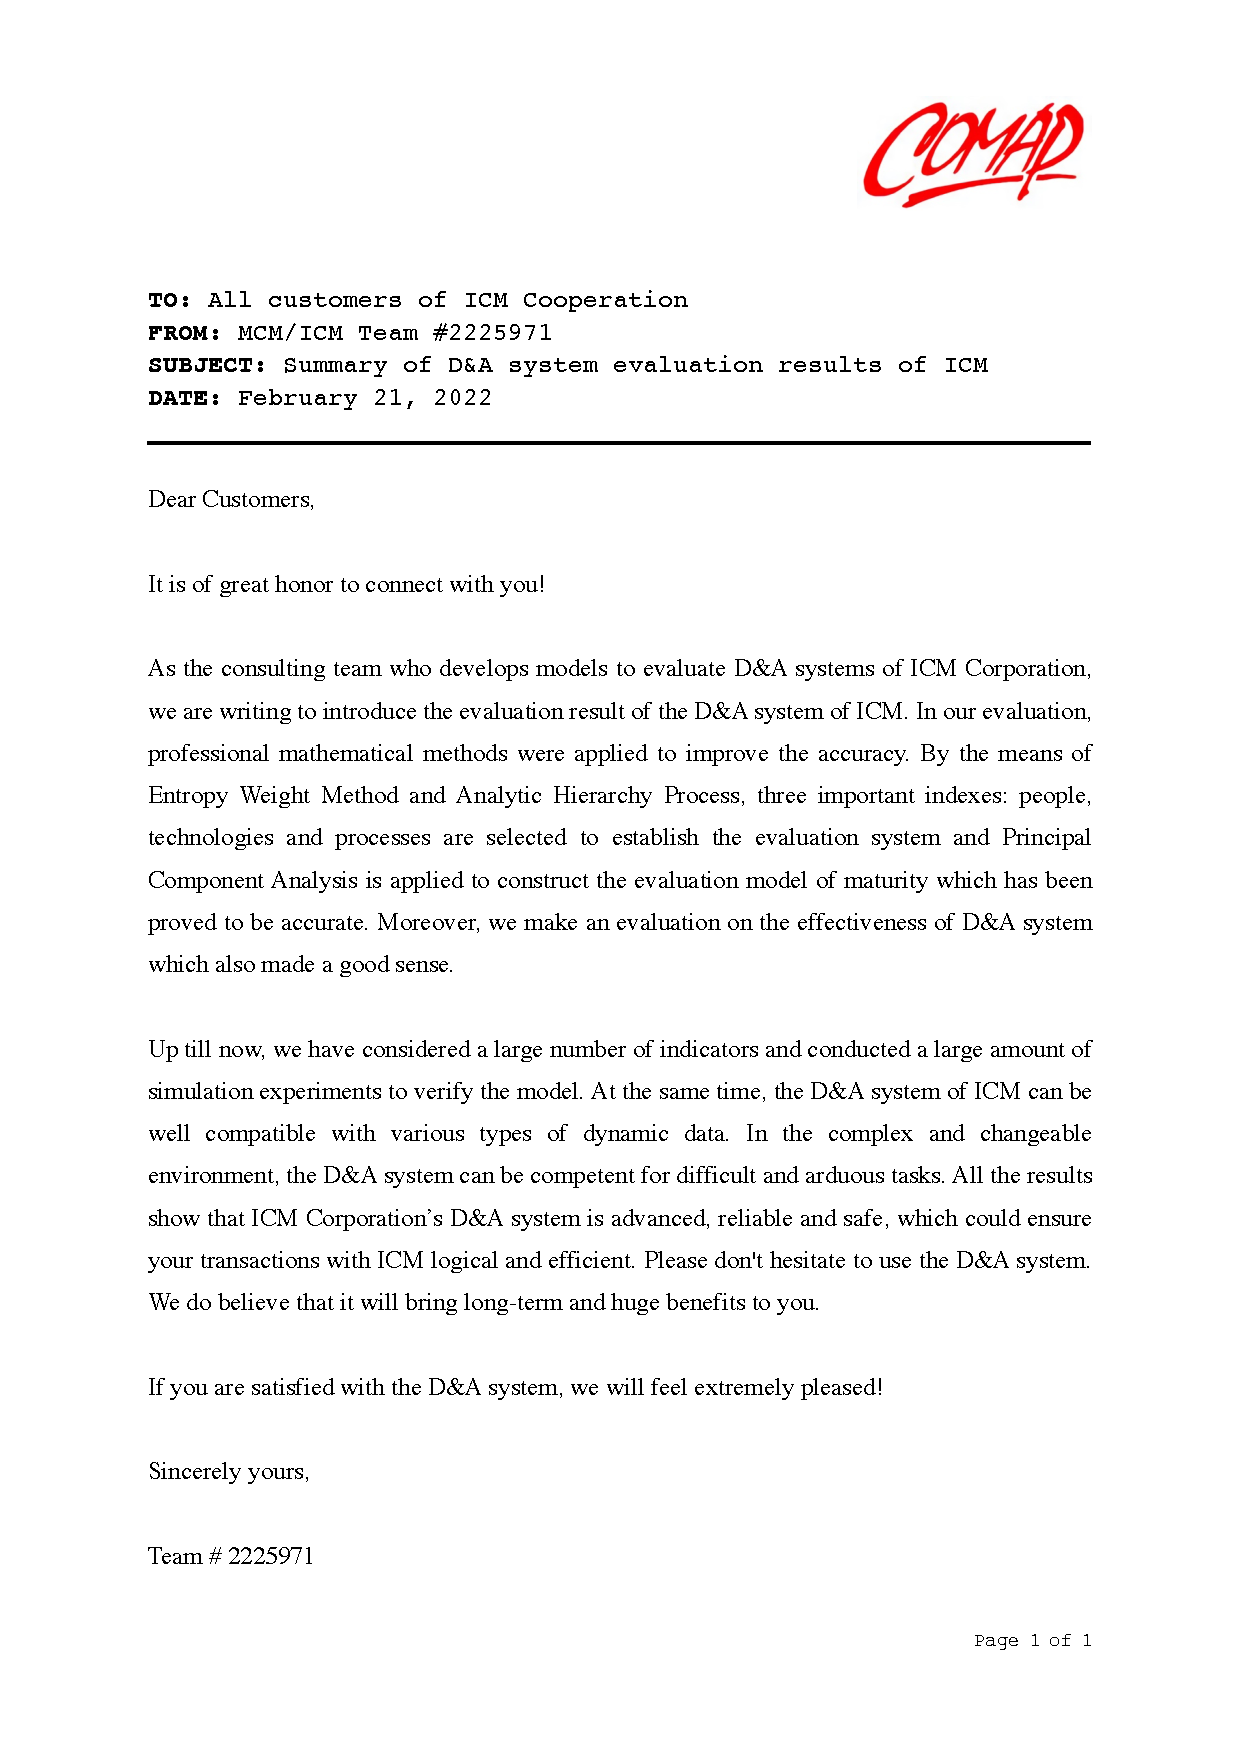
\includepdf{letter.pdf} 
%End
\end{document}